\section{システム実装}
\label{sec:jissou}

\subsection{チーム構成と役割分担}
\label{sec:jissou_team}
本プロジェクトは6名で実施した．役割分担は，作業分解構造（WBS）に基づき，楽曲表現系（ハードウェア全般）を山口・佐藤，楽器系（音色合成・発音機能）を梅野・薄井，通信系（通信同期制御）を宇井・菊池がそれぞれペアで担当する構成とした．
このうち報告者(佐藤)は，ハードウェア面については指揮デバイスの作成，楽器デバイスの受光部回路の作成，および結合テスト時における全体的な調整を担当した．また，ソフトウェア面では，中継機デバイスのLEDMatrixに現在のBPMを表示するDisplayモジュール（Display.h，Display.cpp）の実装を担当した．Displayモジュールのプログラム全文は付録に示す．


\iffalse
計画時に策定した実装フェーズ・テストフェーズのスケジュールを，WBSに基づき週単位に要約したガントチャートを図\ref{fig:gantt_plan}に示す．
期間は2026年5月22日から6月30日までの6週間であり，W1を5月22日の週とする．実装フェーズでは3週目の途中までに各担当の単体作業を完成させ，単体テストは各項目の完成後に順次実施し，3週目以降に結合テストへ移行して4週目末までに全結合テストを完了させる計画とした．6週目は，遅延が生じた場合に結合テストまでを完了させるための予備期間である．

\begin{figure}[htbp]
    \begin{center}
    \begin{ganttchart}[y unit title=0.4cm,
    y unit chart=0.5cm,
    vgrid,hgrid,
    title label anchor/.style={below=-1.6ex},
    title left shift=.05,
    title right shift=-.05,
    title height=1,
    title/.append style={fill=yellow!10},
    progress label text={},
    bar height=0.7,
    group right shift=0,
    group top shift=.6,
    group height=.3]{1}{18}
    %labels
    \gantttitle{6 Weeks（2026/5/22〜6/30）}{18} \\
    \gantttitle{W1}{3}
    \gantttitle{W2}{3}
    \gantttitle{W3}{3}
    \gantttitle{W4}{3}
    \gantttitle{W5}{3}
    \gantttitle{W6}{3}\\
    %tasks
    \ganttbar[bar/.append style={fill=orange!40}]{指揮デバイスの実装/山口・佐藤}{1}{6} \\%elem0
    \ganttbar[bar/.append style={fill=orange!40}]{中継機・受光部の実装/山口・佐藤}{1}{6} \\%elem1
    \ganttbar[bar/.append style={fill=orange!40}]{LEDマトリクス制御の実装/山口・佐藤}{1}{6} \\%elem2
    \ganttbar[bar/.append style={fill=green!40}]{楽器・譜面の実装/梅野・薄井}{1}{6} \\%elem3
    \ganttbar[bar/.append style={fill=green!40}]{音色再現・発音機能の実装/梅野・薄井}{1}{7} \\%elem4
    \ganttbar[bar/.append style={fill=cyan!40}]{通信同期制御の実装/宇井・菊池}{4}{9} \\%elem5
    \ganttbar[bar/.append style={fill=blue!40}]{単体テスト/全員}{4}{12} \\%elem6
    \ganttbar[bar/.append style={fill=blue!40}]{結合テスト/全員}{7}{15} \\%elem7
    \ganttbar[bar/.append style={fill=red!40}]{予備期間/全員}{16}{18}%elem8

    %relations
    \ganttlink{elem0}{elem6}
    \ganttlink{elem3}{elem6}
    \ganttlink{elem5}{elem6}
    \ganttlink{elem6}{elem7}
    \ganttlink{elem7}{elem8}
    \end{ganttchart}
    \end{center}
    \caption{計画時のスケジュール（実装フェーズ・テストフェーズの週単位要約）}
    \label{fig:gantt_plan}
\end{figure}

\fi

また，計画当初のガントチャートを図\ref{fig:gantt_zissou}，最終的な実績のガントチャートを図\ref{fig:gantt_final}に示す．
図\ref{fig:gantt_final}は，WBSの各タスクについて，実際に作業を行った期間と作業達成率を日単位で示したものである．
ハードウェア面については，部品の変更や仕様の変更などによって大幅に作業が遅延した．この遅延により，プロジェクト全体として遅延傾向になったと考える．


\begin{figure}[htbp]
    \centering
    \includegraphics[width=\textwidth]{figs/GC_honto_zissou.png}
    \caption{計画書時点のガントチャート（上段：実装，下段：テスト）}
    \label{fig:gantt_zissou}
\end{figure}


% \begin{figure}[htbp]
%     \centering
%     \includegraphics[width=\textwidth]{figs/GC_decide_test.png}
%     \caption{計画書時点のガントチャート(テスト)}
%     \label{fig:gantt_test}
% \end{figure}


\begin{figure}[htbp]
    \centering
    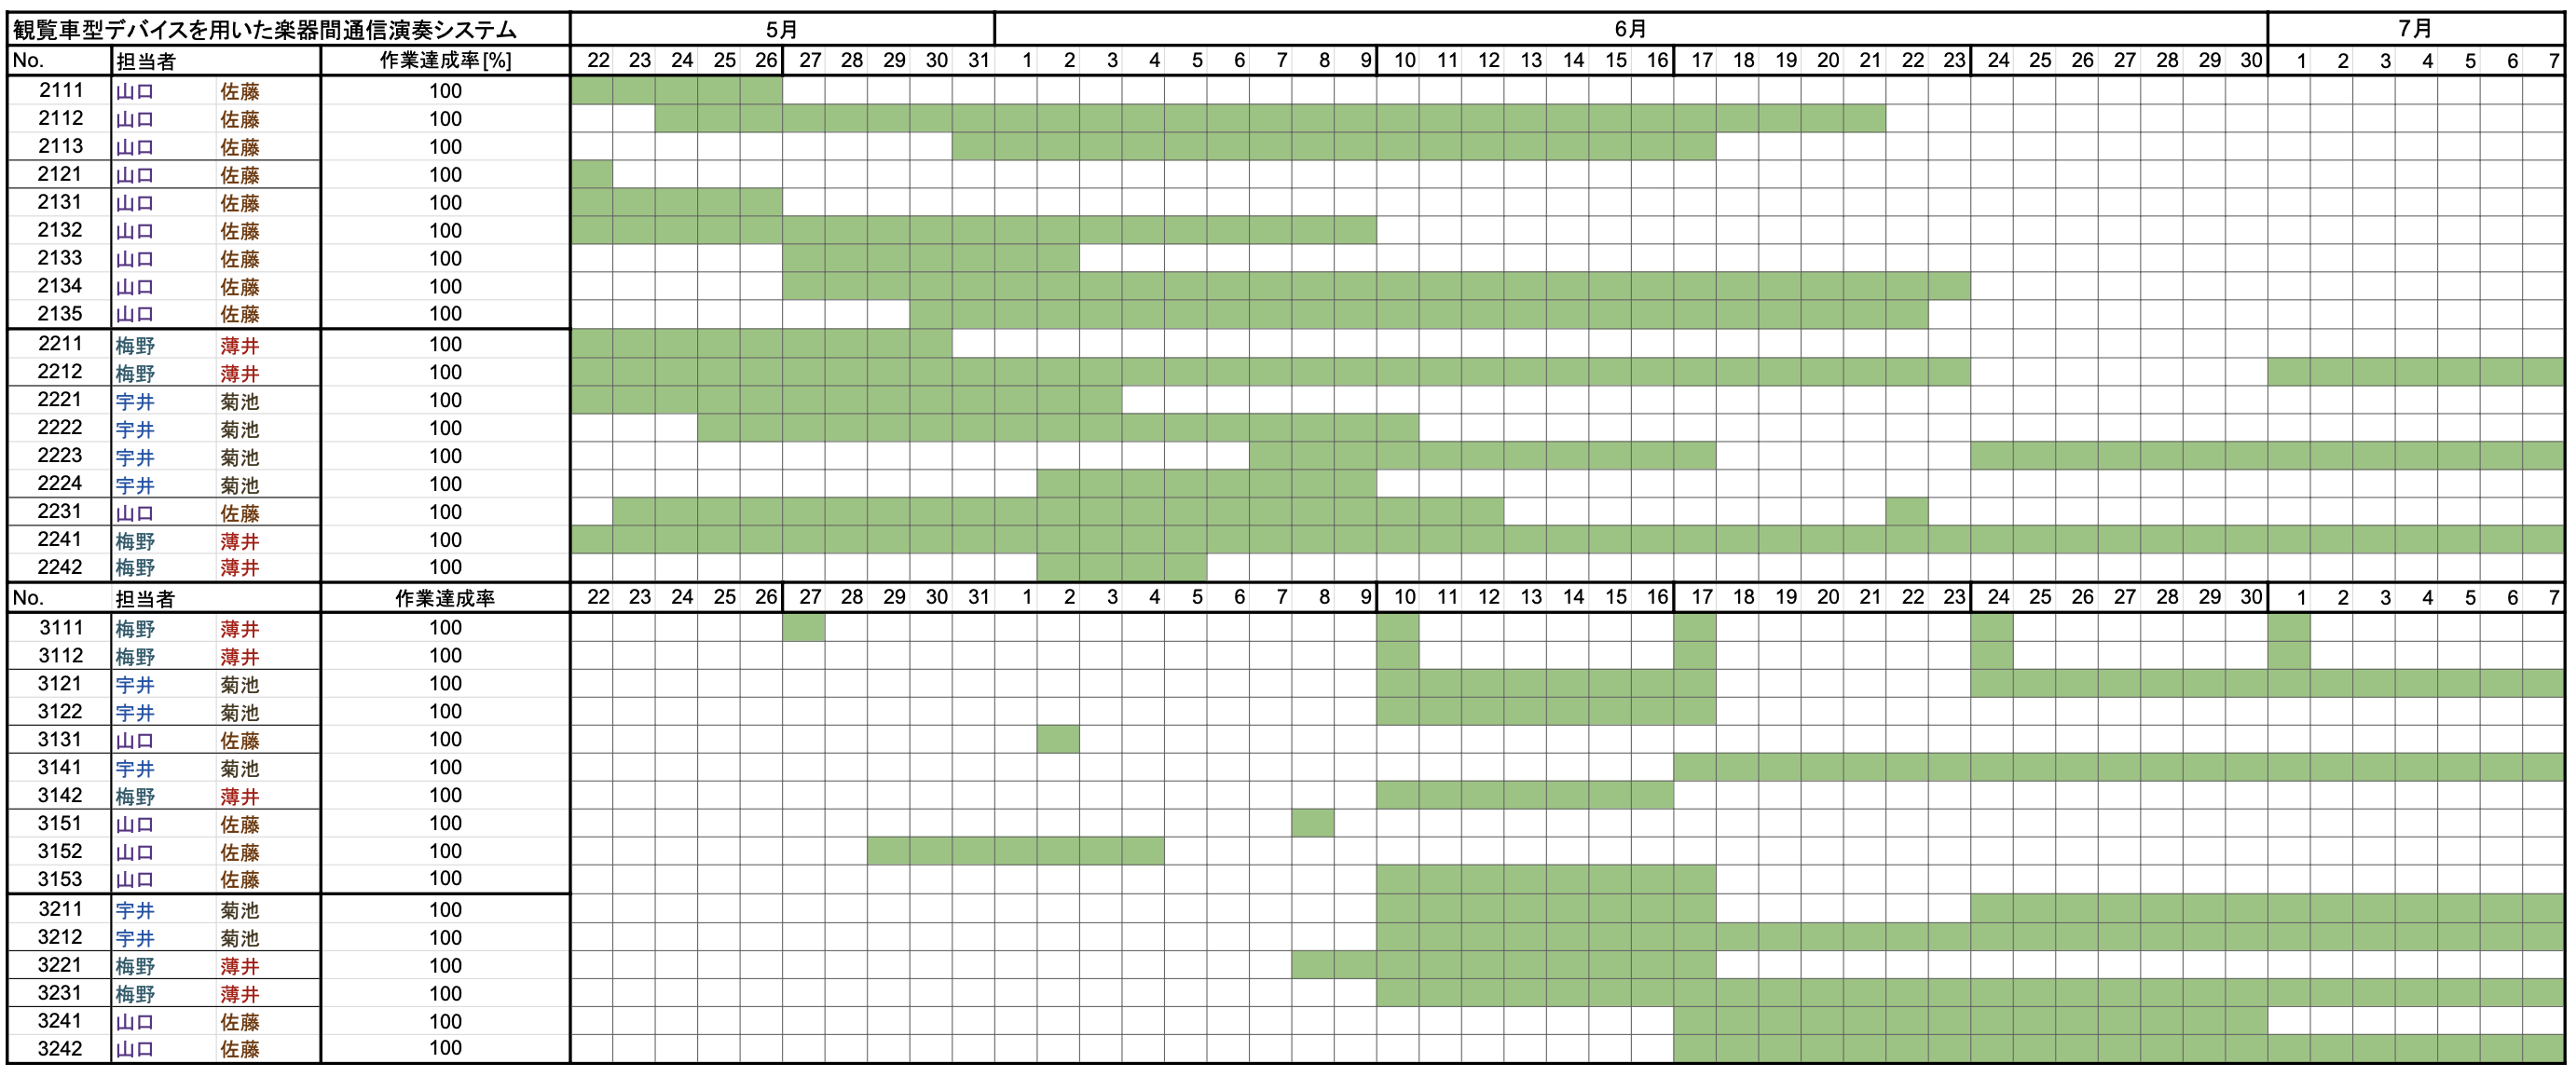
\includegraphics[width=\textwidth]{figs/GC_decide_goal.png}
    \caption{最終的な実績のガントチャート（上段：実装，下段：テスト）}
    \label{fig:gantt_final}
\end{figure}
\FloatBarrier

\subsection{報告者の担当範囲と技術的課題}
本節では，報告者が担当したハードウェアの実装について，採用した技術の選定理由を述べたうえで，実装の過程で直面した技術的課題とその解決のために行った技術的貢献を，各デバイスごとに説明する．
ハードウェア実装における共通の課題は，設計上は動作するはずの回路や機構を，実環境において安定して動作させることであった．具体的には，回転体の質量バランスや軸の摩擦といった機械的な問題，モータの特性変動といった電気的な問題，およびレーザー光の受光精度という光学的な問題が，実装段階ではじめて顕在化した．
以下では，これらの課題に対して行った対応を含めて述べる．


\FloatBarrier

\subsubsection{指揮デバイス}
\label{sec:jissou_siki}

はじめに，操作入力部品の選定理由について述べる．BPM・音量の調整には，スライド式可変抵抗器を採用した．回転式の可変抵抗器と比較して選定した理由は次の2点である．第一に，つまみの物理的な位置が設定値と対応するため，ユーザが現在のBPM・音量の段階を，表示装置を介さずつまみの位置のみから確認できるためである．
第二に，本デバイスは「指揮棒を振っている」というユーザの操作によって演奏が変化することで没入感を高めることが目的であり，回転式と比較してスライド式はデバイスを握ったまま親指のみで容易に操作が可能であり，演奏中に持ち替えを必要としないためである．
また，抵抗値には\SI{10}{\kilo\ohm}を選定した．これは，分圧回路としてArduinoのアナログ入力へ接続する際に，消費電流を抑えつつ，アナログ/デジタル変換の入力インピーダンスに対して十分に低い出力インピーダンスを保てる標準的な値である．

次に，振り動作の検知に用いる加速度センサの選定理由について述べる．振り動作の検知には，デジタル3軸加速度センサADXL345を採用した．選定理由は次の3点である．
第一に，3軸の加速度を同時に計測できるため，3軸のベクトル合成値を判定に用いることで，ユーザがデバイスを振る方向に依存しない検知を実現できる．第二に，このモジュールはI2C通信に対応しており，信号線2本（SDA・SCL）でArduinoと接続できるため，限られた実装空間における配線数を削減できる．第三に，測定レンジを$\pm 2g$から$\pm 16g$まで設定でき，振り動作で生じる加速度に対して測定値の飽和を避けた計測ができる．加えて，割り込み信号の出力ピン（INT1）を備えており，閾値超過の検知をセンサ側で行いArduinoへ通知する構成に対応できる．

次に，実装における技術的貢献について述べる．実装した指揮デバイスの内部を図\ref{fig:r_sikiin}に，外装を含む完成状態を図\ref{fig:r_siki}に示す．
内部は，ブレッドボード上にタクトスイッチと加速度センサを実装し，2系統のスライド式可変抵抗器はユニバーサル基板へはんだ付けして固定した．
外装の設計にあたっては，ユーザビリティの向上を目的として，ユーザが操作するスライド式可変抵抗器のスライダー部分およびタクトスイッチの部分を外装から露出させる構造とした．なお，本稿ではユーザが操作方法の説明を受けなくても，操作箇所を特定し目的の操作を行える度合いをユーザビリティと定義している．
これにより，ユーザは外装を開けることなく，露出したつまみとボタンのみで演奏の開始・終了とBPM・音量の全操作が行える．

\begin{figure}[htbp]
  \centering
  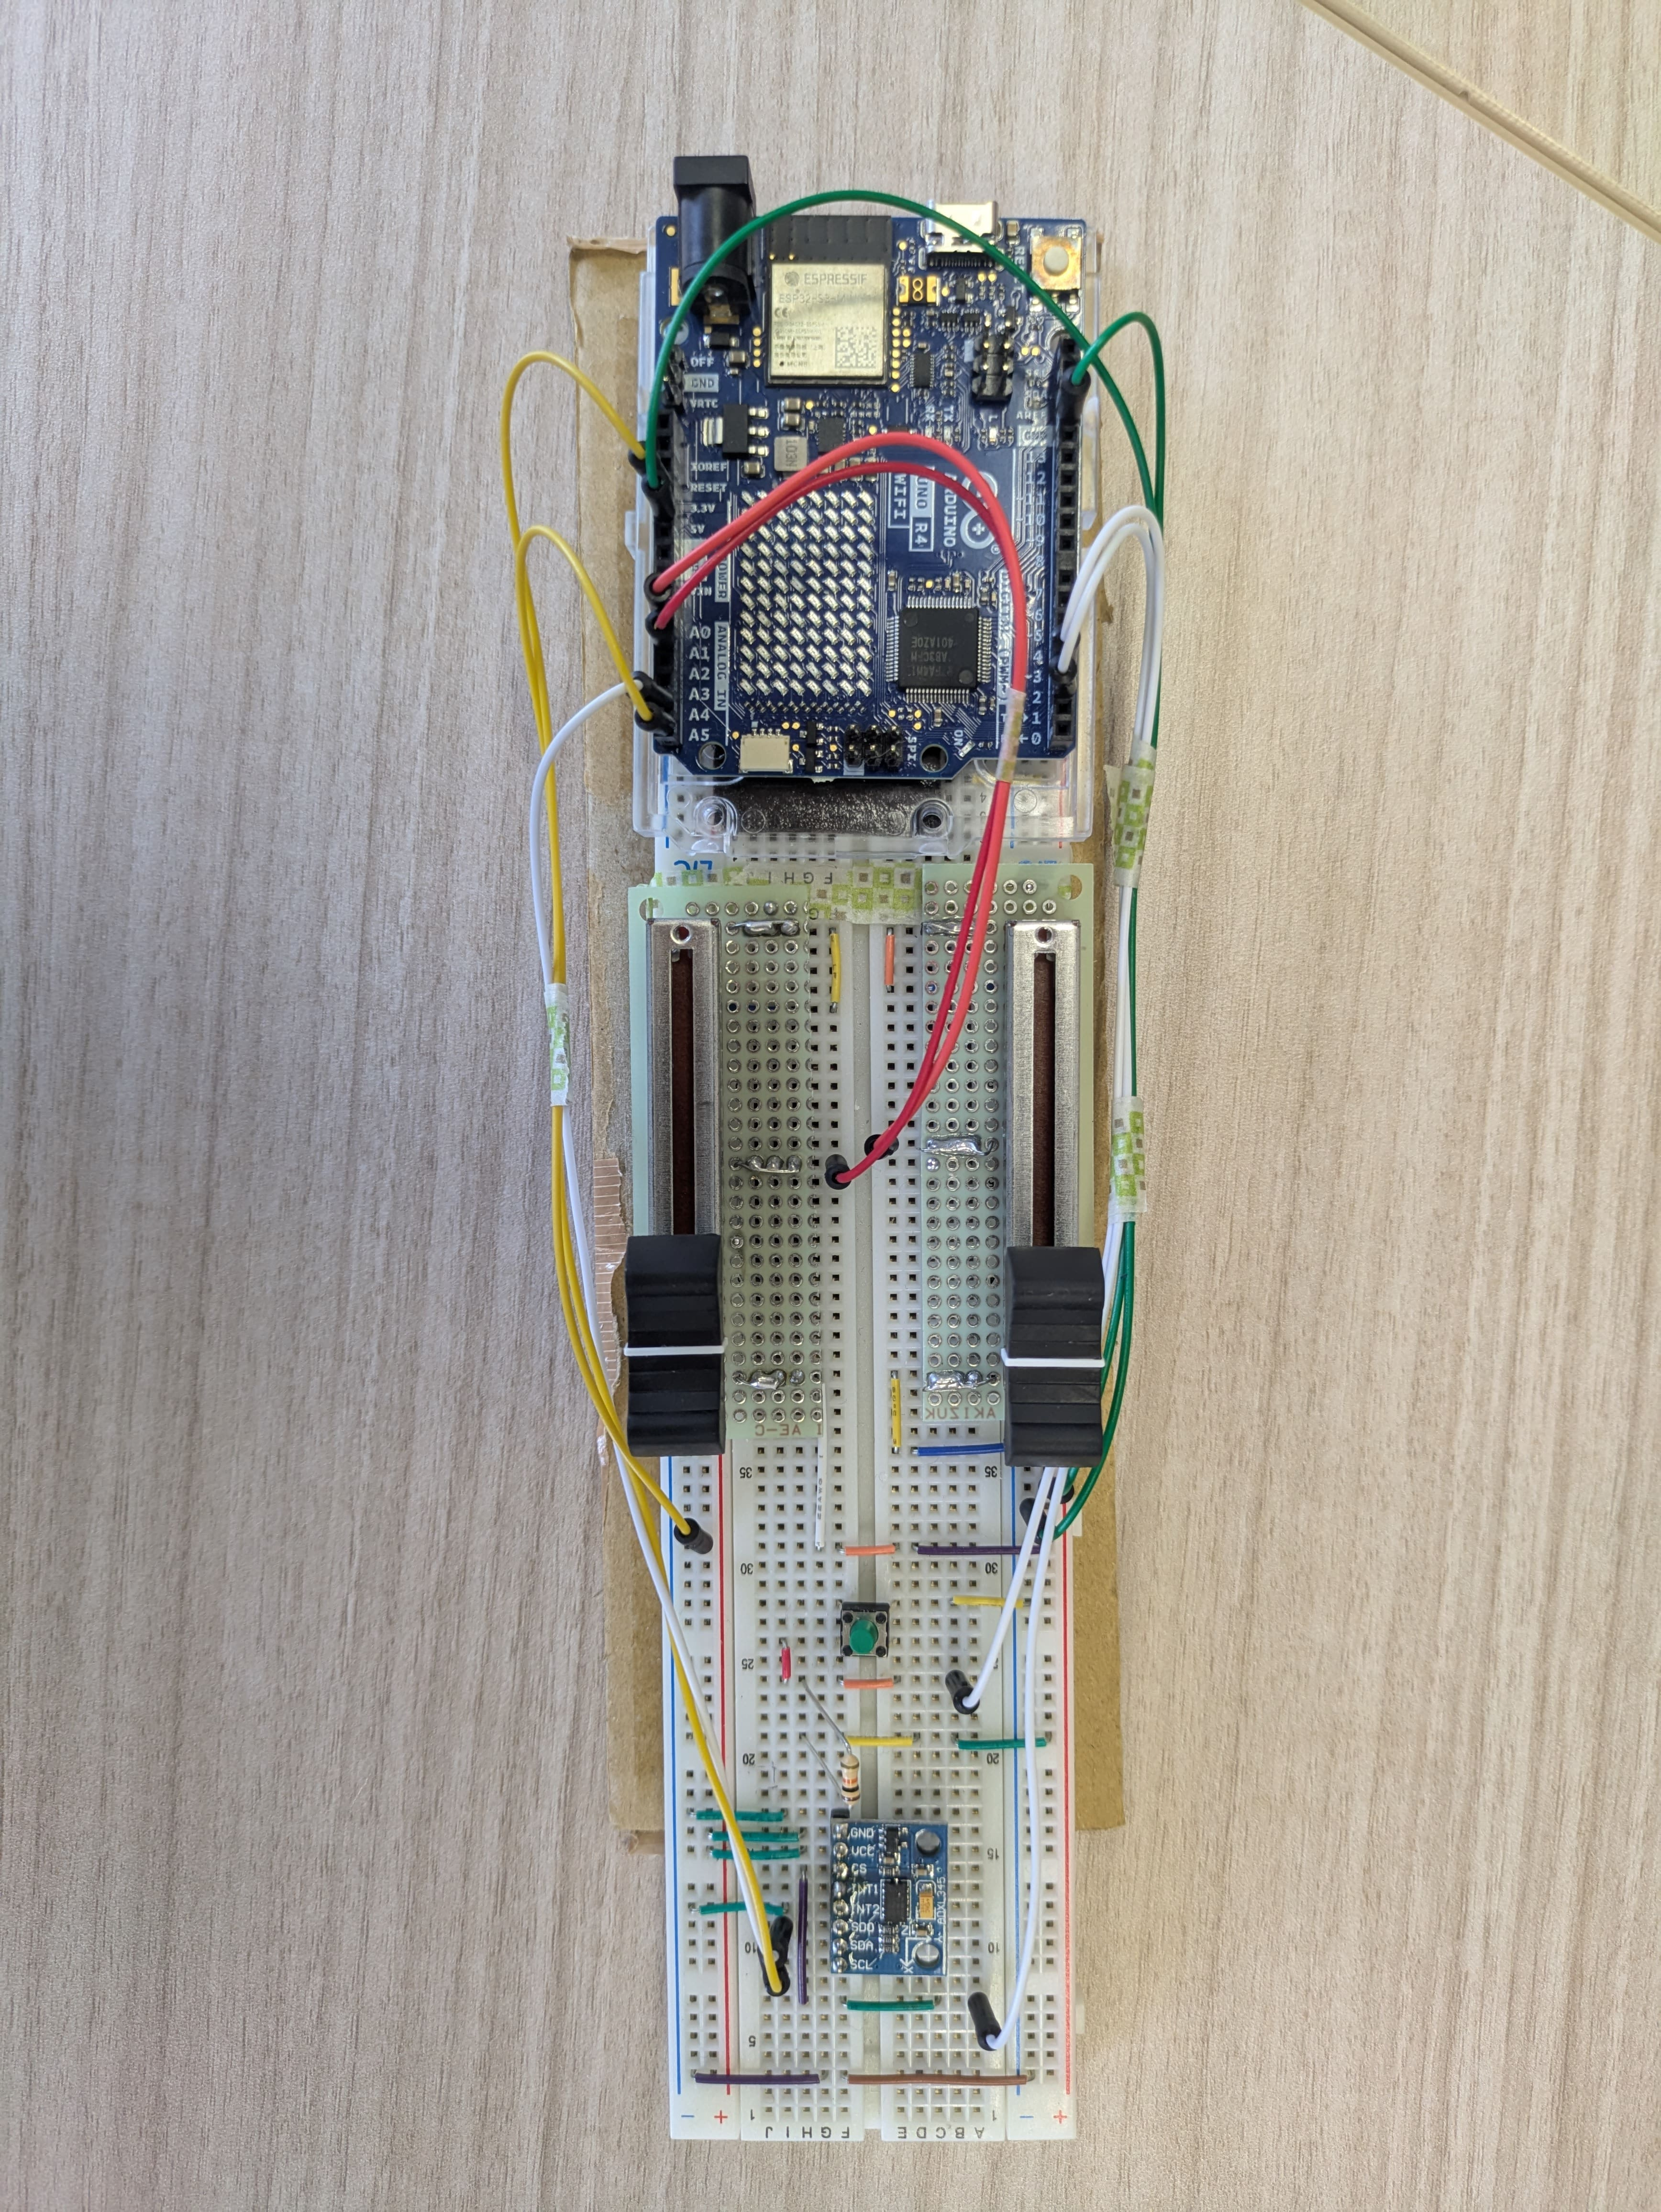
\includegraphics[width=0.55\textwidth]{figs/R_sikiin.jpg}
  \caption{指揮デバイスの内部実装}
  \label{fig:r_sikiin}
\end{figure}

\begin{figure}[htbp]
  \centering
  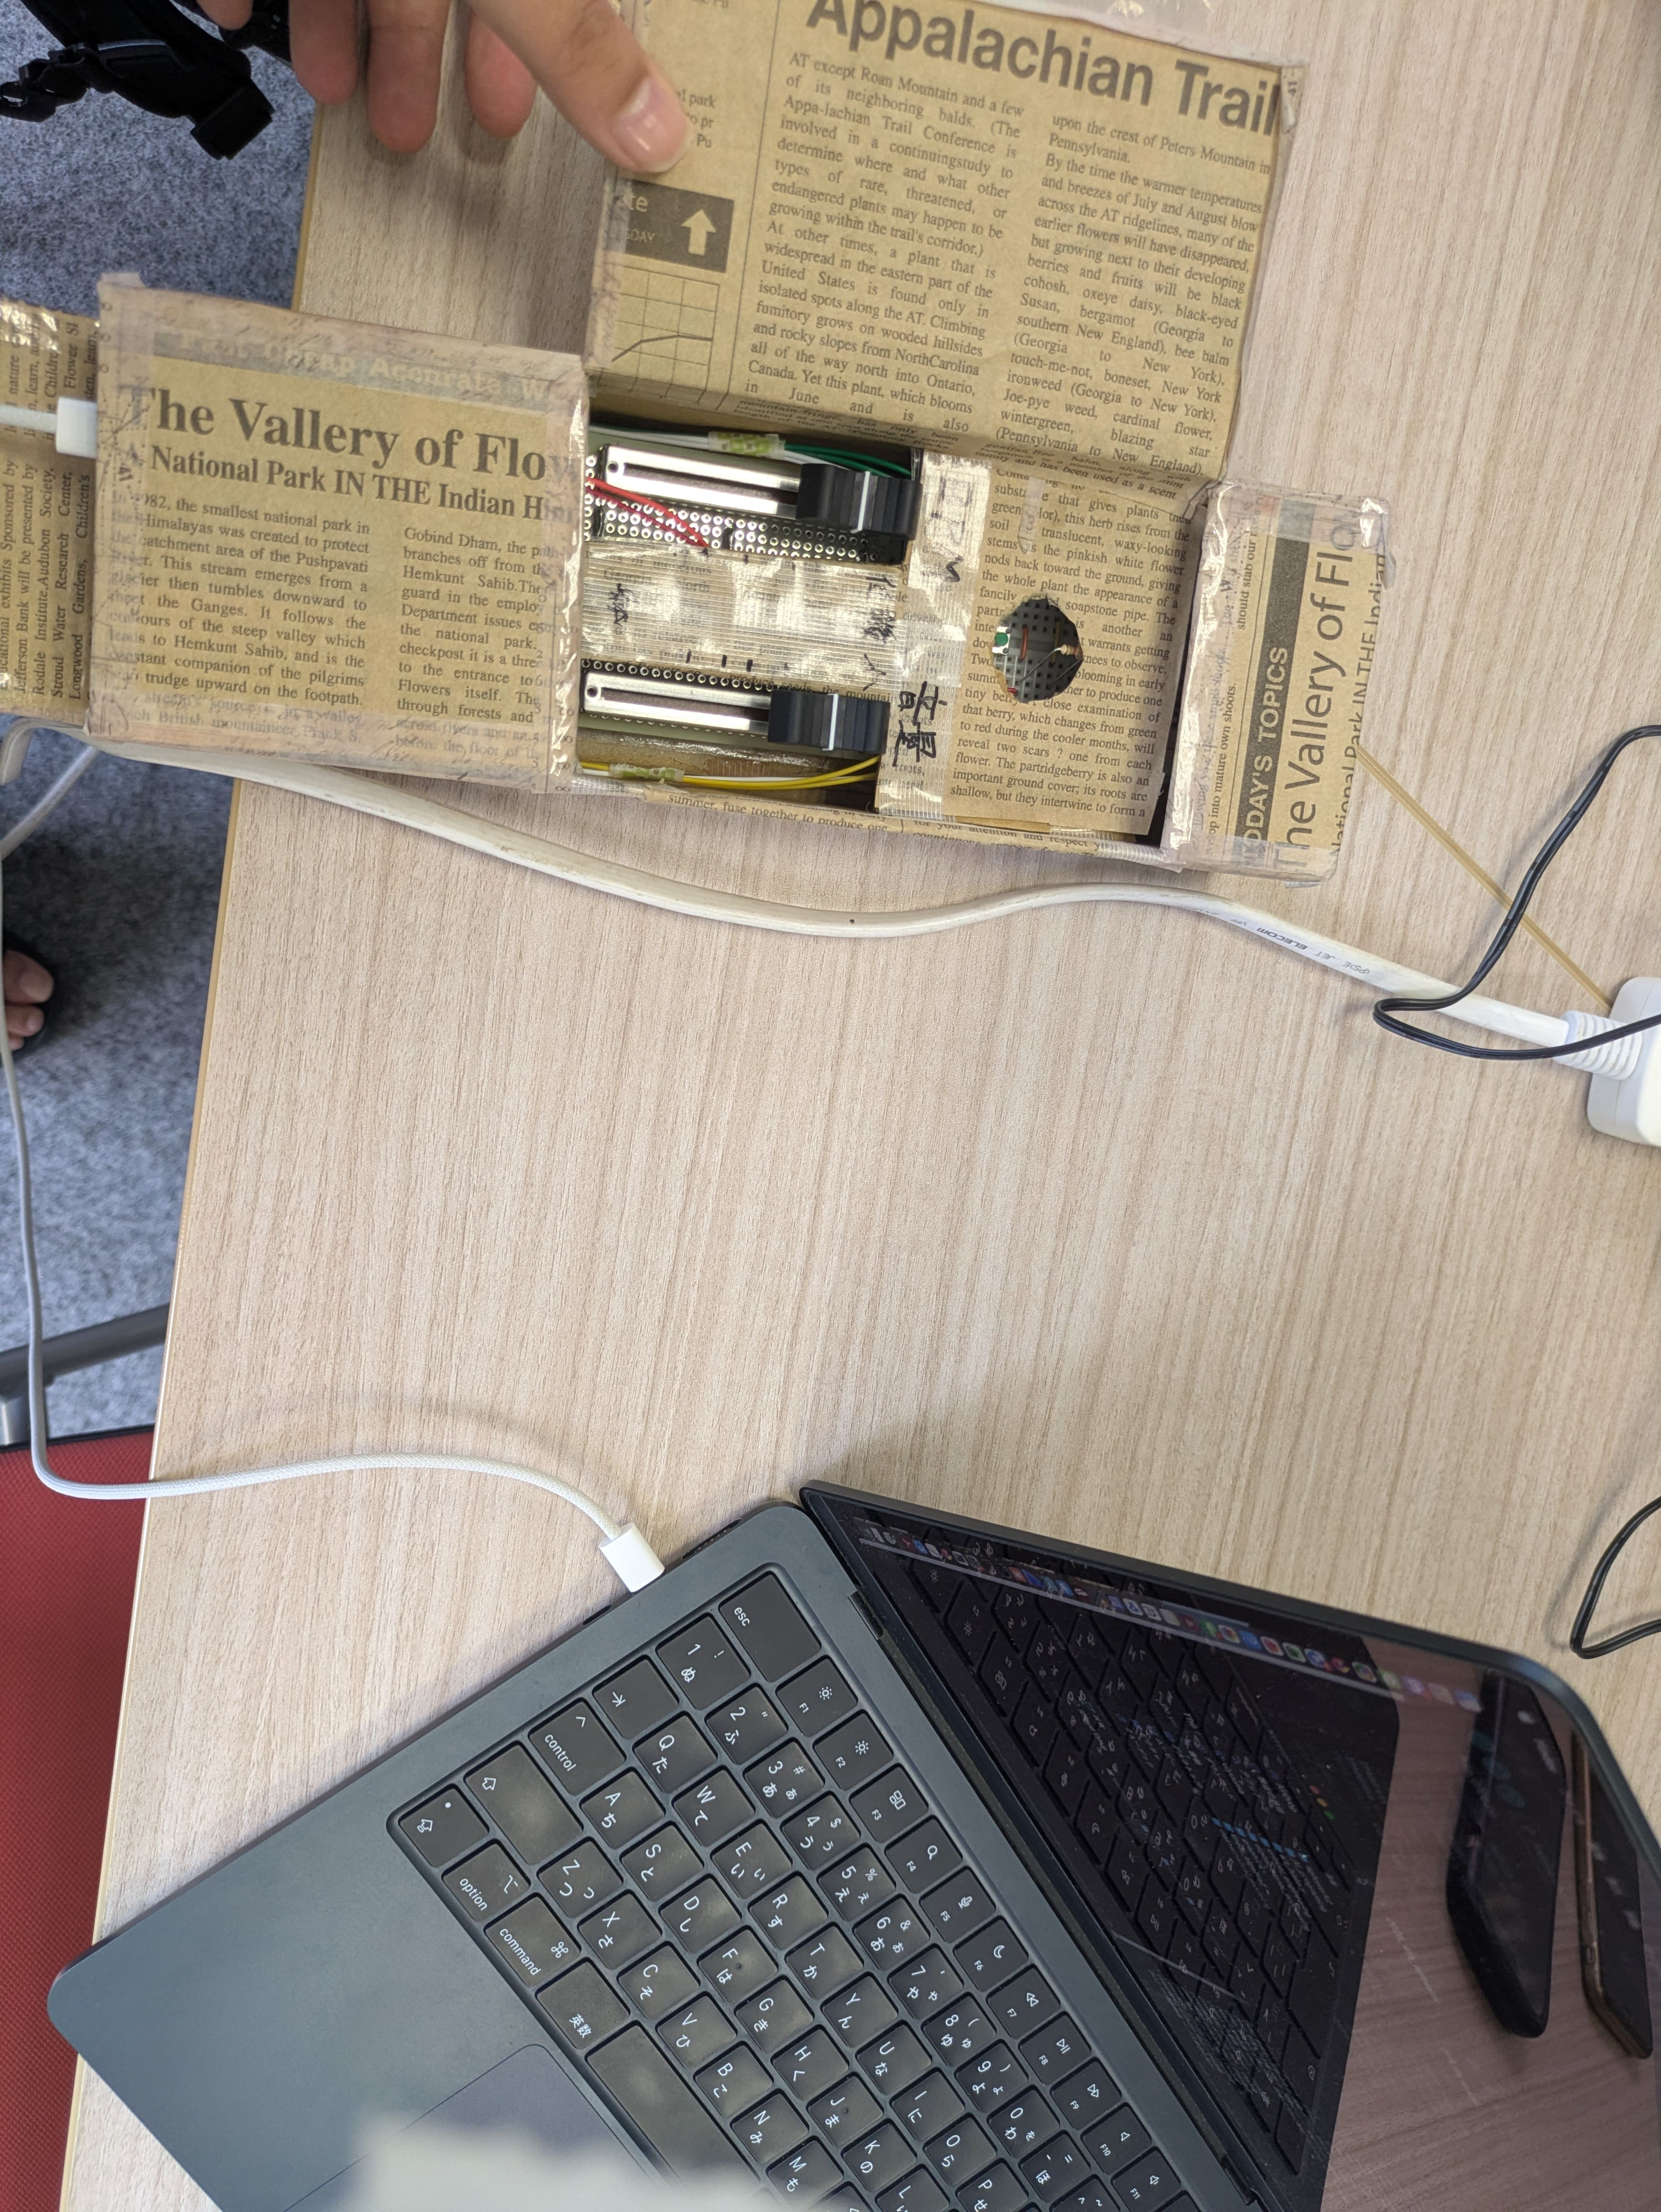
\includegraphics[width=0.7\textwidth]{figs/R_siki.jpg}
  \caption{作成した指揮デバイス}
  \label{fig:r_siki}
\end{figure}

\FloatBarrier



\subsubsection{観覧車型中継機デバイス}
\label{sec:jissou_kan}

はじめに，主要部品の選定理由について述べる．
第一に，回転リング上のレーザーモジュールの電源には，ボタン電池を採用した．
レーザーモジュールは回転リングに搭載されて本体ごと回転するため，外部から配線で給電すると回転に伴い配線が捻れ，回転体へ電力を伝えるための回転接点部品であるスリップリング等の追加機構が必要となる．
そこで，電源を回転体上で完結させる方式とし，回転体に搭載する電源として小型・軽量で質量バランスへの影響が小さいボタン電池を選定した．型番には，ボタン電池の中でも大容量なCR2477を選定した．採用したレーザーモジュールは\SI{3}{V}駆動かつ定電流回路を内蔵しているため，公称電圧\SI{3}{V}で外部抵抗なしに直結でき，回路を簡素化できる\cite{laser}．また，基板取付用ホルダーを介して実装することで，電池の消耗時に交換が可能である．
実際に作成したレーザーによる光信号送信基盤を図\ref{fig:laser_kiban}に示す．図\ref{fig:laser_kiban}の通り，ユニバーサル基盤にボタン電池ホルダとレーザーモジュールをはんだ付けしている．これにより，ボタンをオンにすると回転リングの穴からレーザー光が照射される．

第二に，モータの駆動には，モータドライバモジュールを採用した．Arduinoのデジタル出力ピンはモータの駆動に必要な電流を直接供給できないため，Arduinoからモータへ電力を供給するためのモータドライバが必要となる．DRV8835を選定した理由は次の3点である．
第一に，Hブリッジという4つのスイッチング素子を組み合わせ，モータへ流す電流の向きを切り替えられる回路を内蔵し，PWM信号の入力によって回転速度の制御が可能であるからだ．第二に，モータ用電源として最大\SI{11}{V}・1チャネルあたり最大\SI{1.5}{A}の駆動に対応しており，ACアダプタからの\SI{5}{V}単一電源系でギヤボックスモータを駆動できる．第三に，ブレッドボードに直接実装できる小型のDIP化モジュールであり，試作段階においてはんだ付けを行わずに配線を変更できる．実装したモータドライバ周辺の回路を図\ref{fig:r_mota}に示す．

\begin{figure}[htbp]
    \centering
    \includegraphics[width=0.6\textwidth]{figs/R_laser.jpg}
    \caption{実際に作成したレーザーによる光信号送信基盤}
    \label{fig:laser_kiban}
\end{figure}



\begin{figure}[htbp]
  \centering
  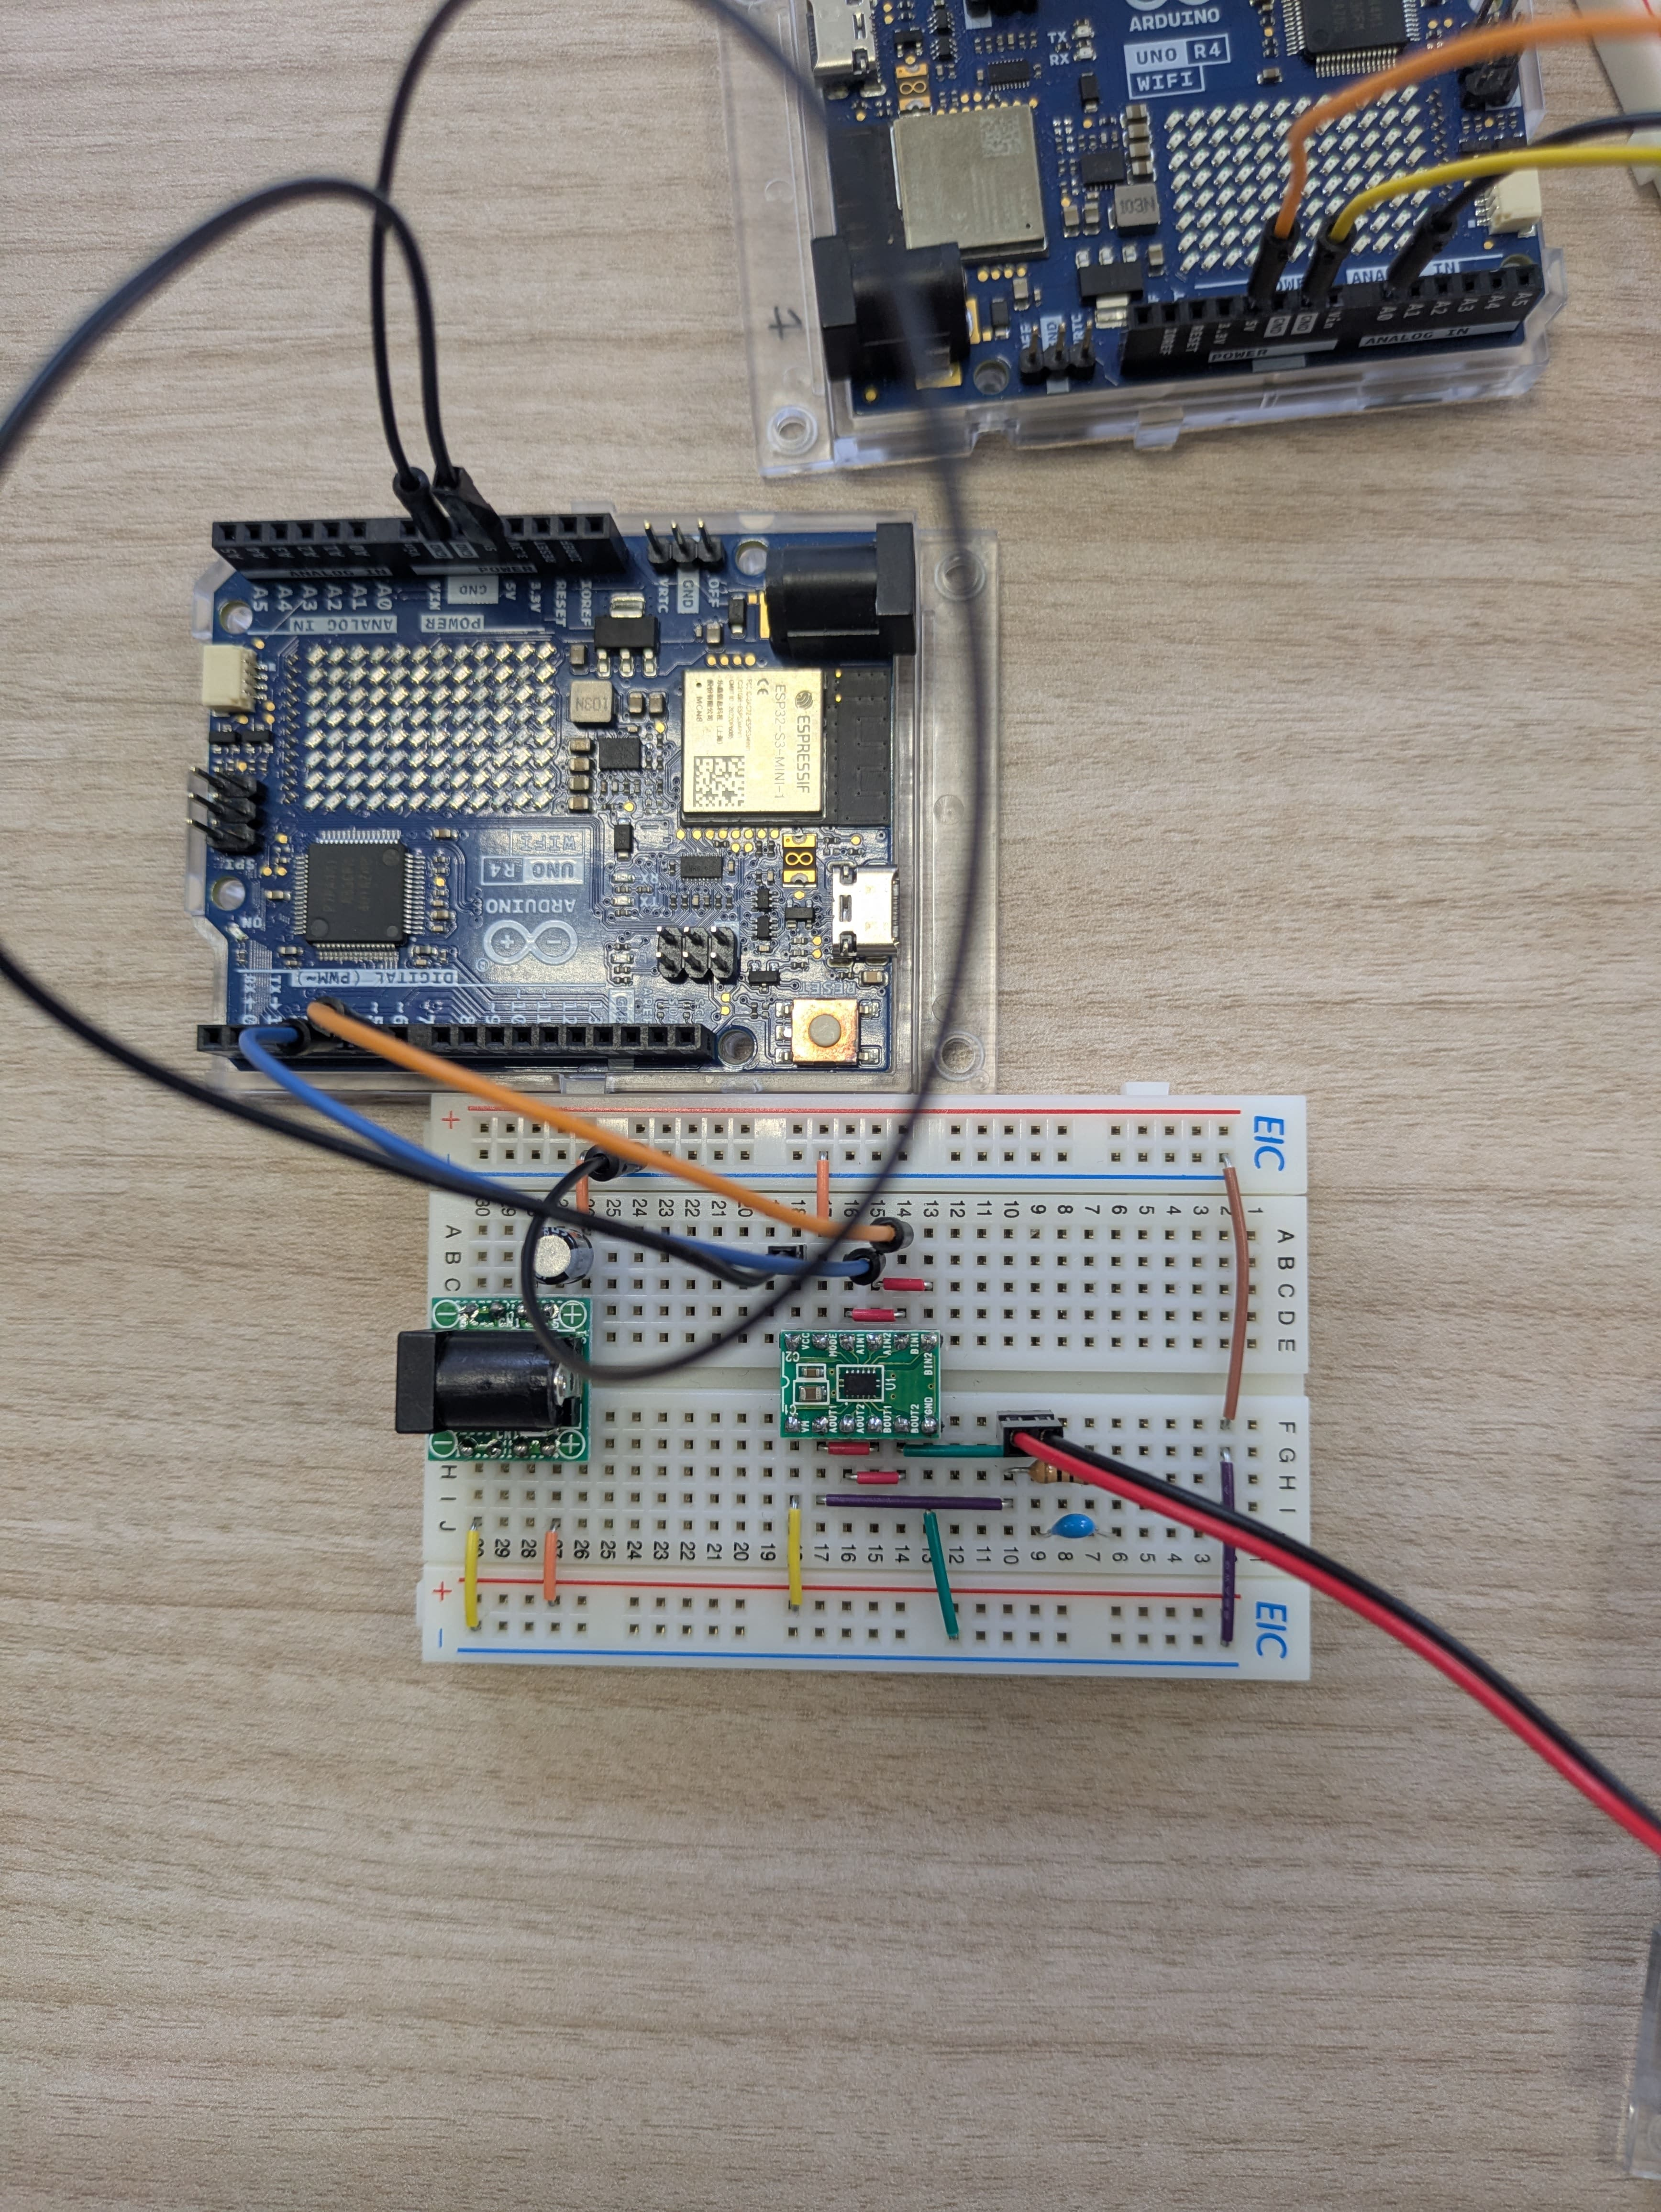
\includegraphics[width=0.6\textwidth]{figs/R_mota.jpg}
  \caption{モータドライバ周辺の回路実装}
  \label{fig:r_mota}
\end{figure}

次に，実装における技術的貢献について説明する．実装した中継機デバイスの全体を図\ref{fig:r_zentai}に示す．

\begin{figure}[htbp]
  \centering
  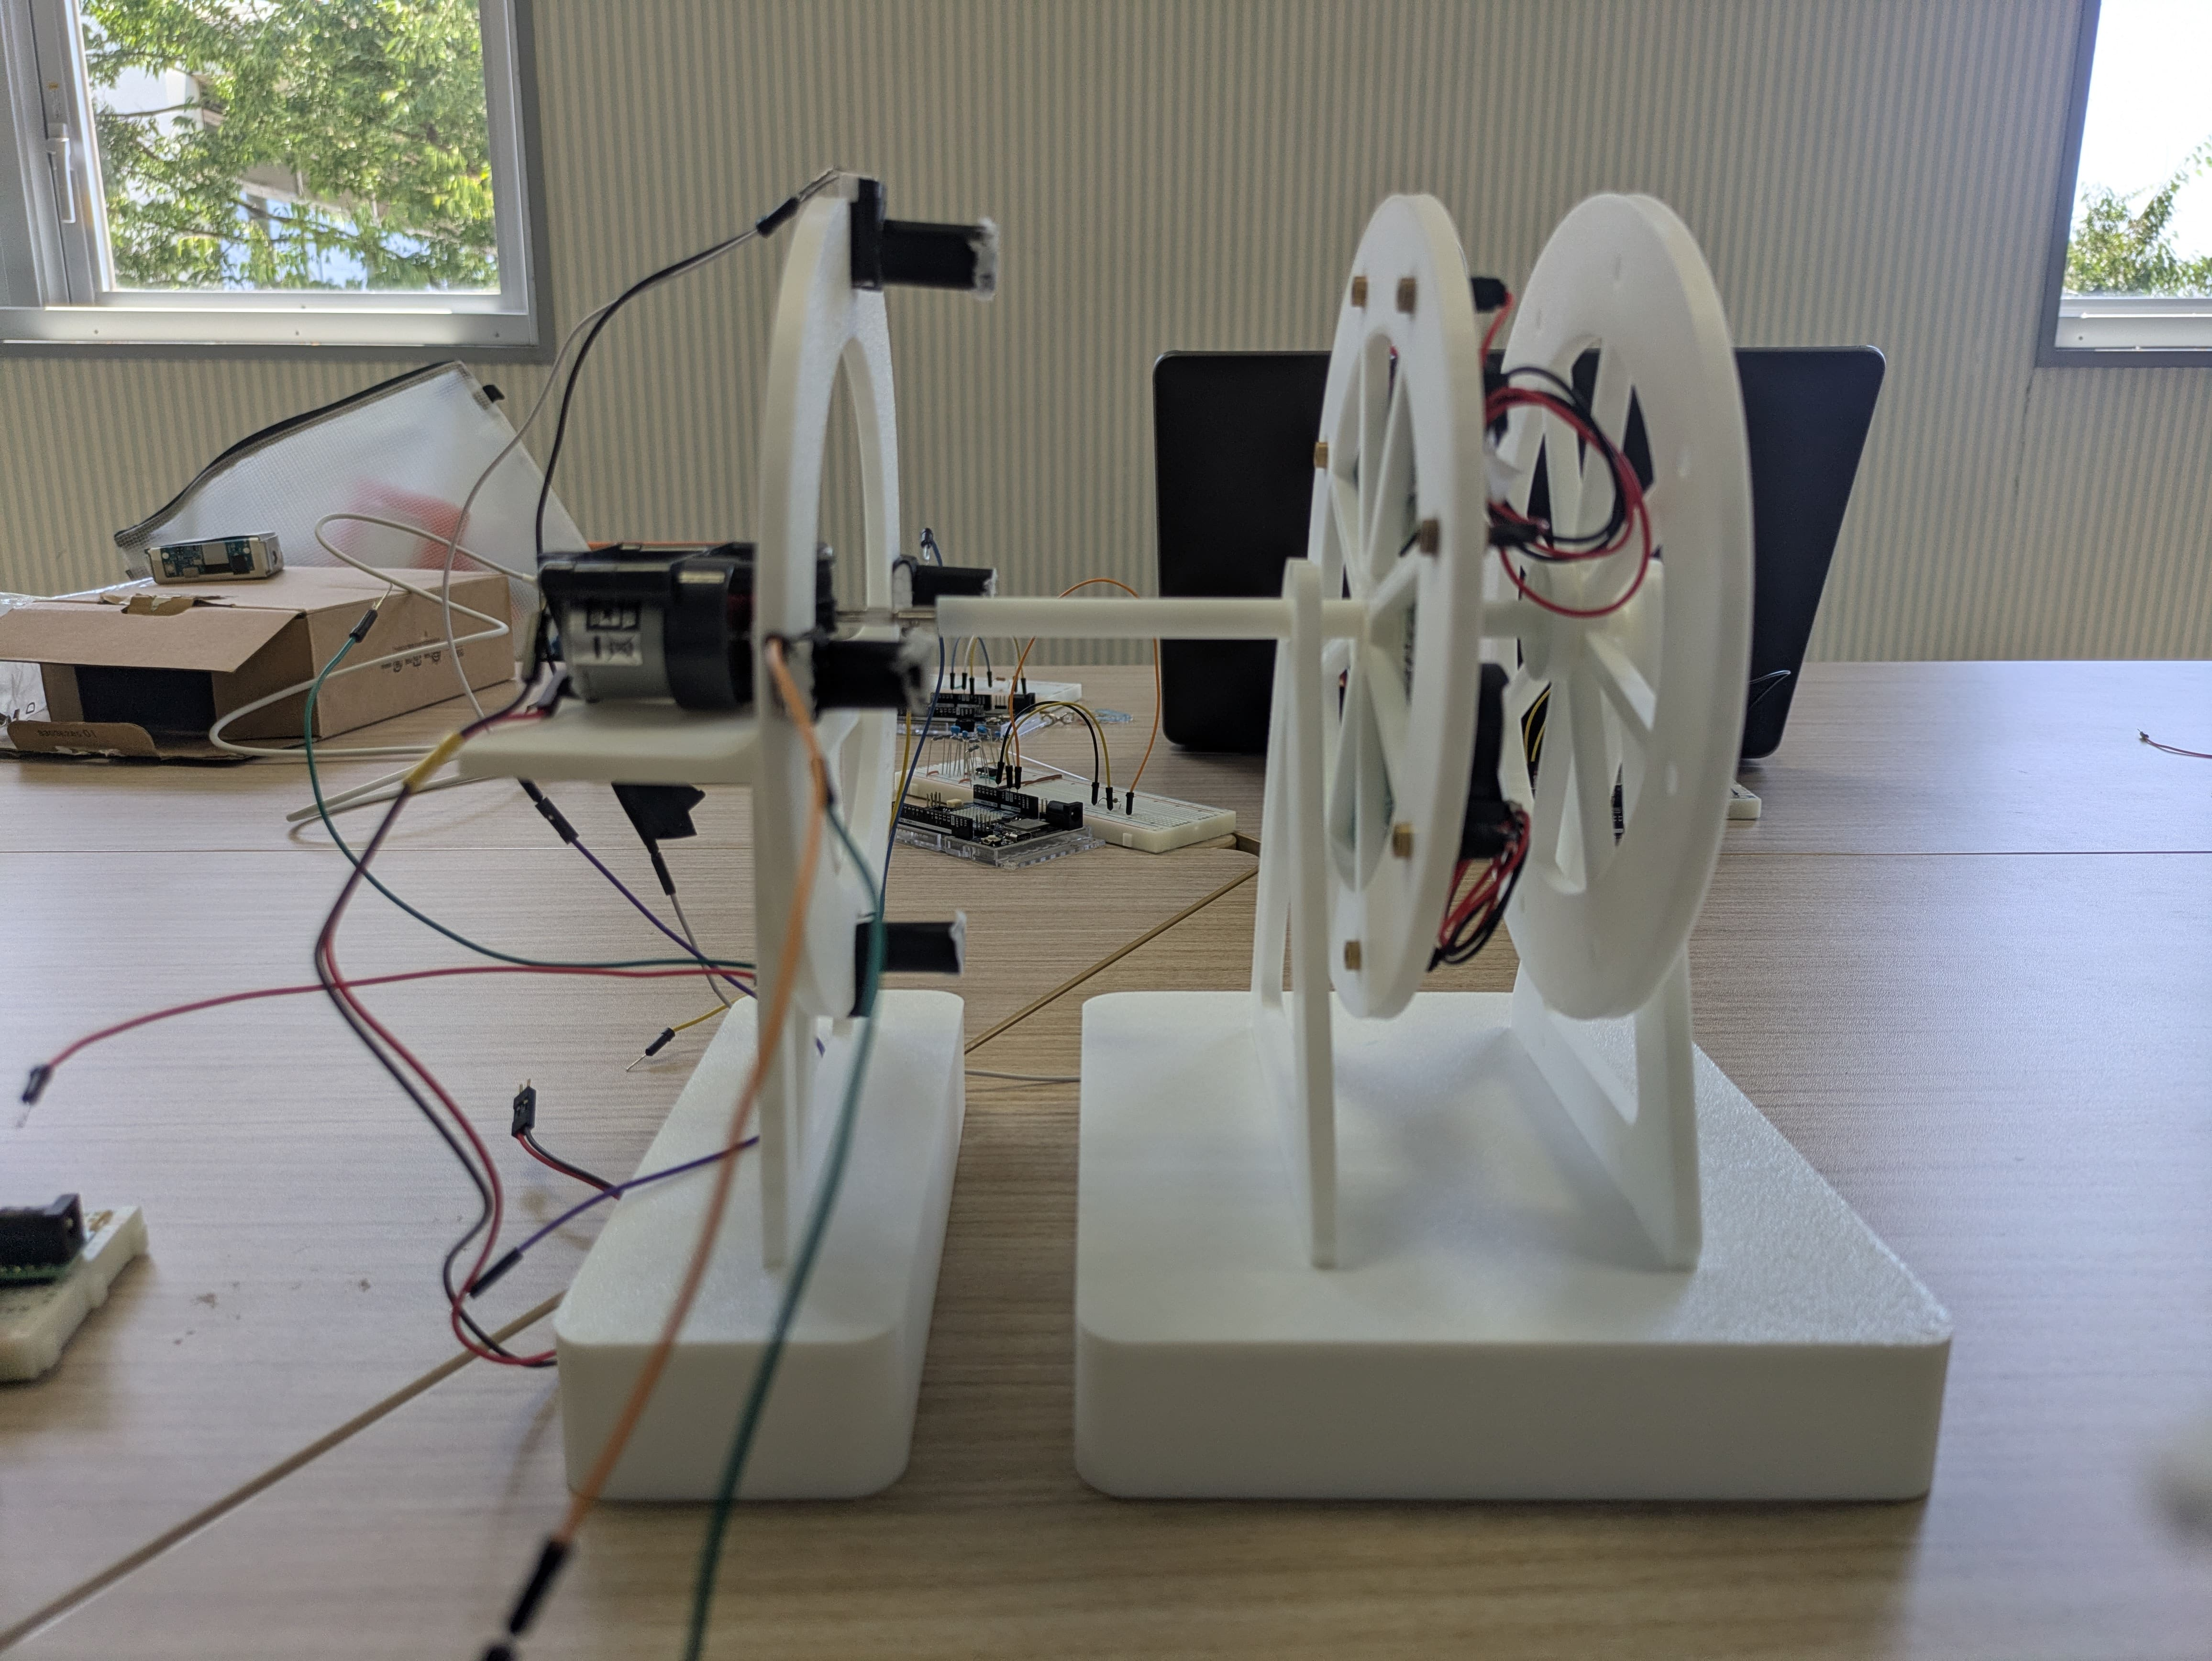
\includegraphics[width=0.8\textwidth]{figs/R_zentai.jpg}
  \caption{実装した中継機デバイスの全体（左：受光部リング側，右：回転リング側）}
  \label{fig:r_zentai}
\end{figure}

\noindent
まず，回転部の機械的な安定化について述べる．回転する部品を支える回転軸は，安定性を担保するために左右の支柱で軸受け穴の大きさを非対称とし，ギヤボックスモータに接続する側の穴を大きくしている．これは，モータ側の軸受けに回転トルクによる負荷が集中し，穴の径が小さいと軸が折れるおそれがあるためである．
軸まわりの部品形状を図\ref{kanran2}，図\ref{kanran3}に示す．計画書当初は同一の大きさに軸を設計しており，実際に3Dプリンターにて実装をしたところ耐久性に乏しく折れてしまったが，現在の仕様に変更したところ実験中に軸が折れることはなく，安定性が担保された．
さらに，軸受け部にはグリス（半固体状の潤滑剤）を塗布し，軸と軸受け間の摩擦を低減させた．また，回転軸をモータへ差し込む接続部にはネジロック剤（振動による締結部の緩みを防止する接着剤）を塗布し，回転の振動による軸の緩み・脱落を防止した．

% \begin{figure}[htbp]
%   \centering
%   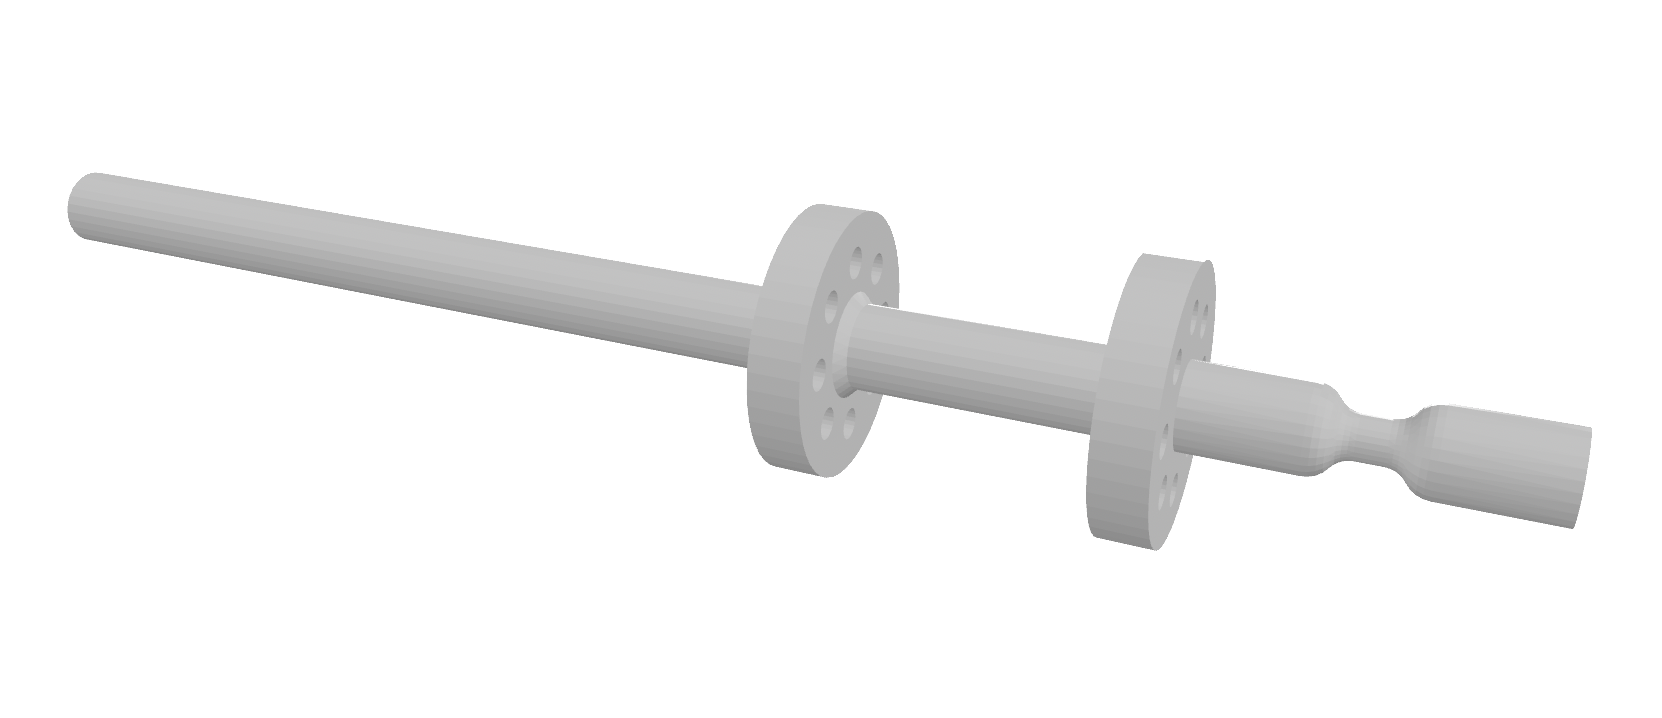
\includegraphics[width=0.45\textwidth]{figs/model_shaft.png}
%   \caption{回転軸部の形状（3Dモデルデータ）}
%   \label{fig:jiku_daiyou}
% \end{figure}

% \begin{figure}[htbp]
%     \centering
%     \centering
%     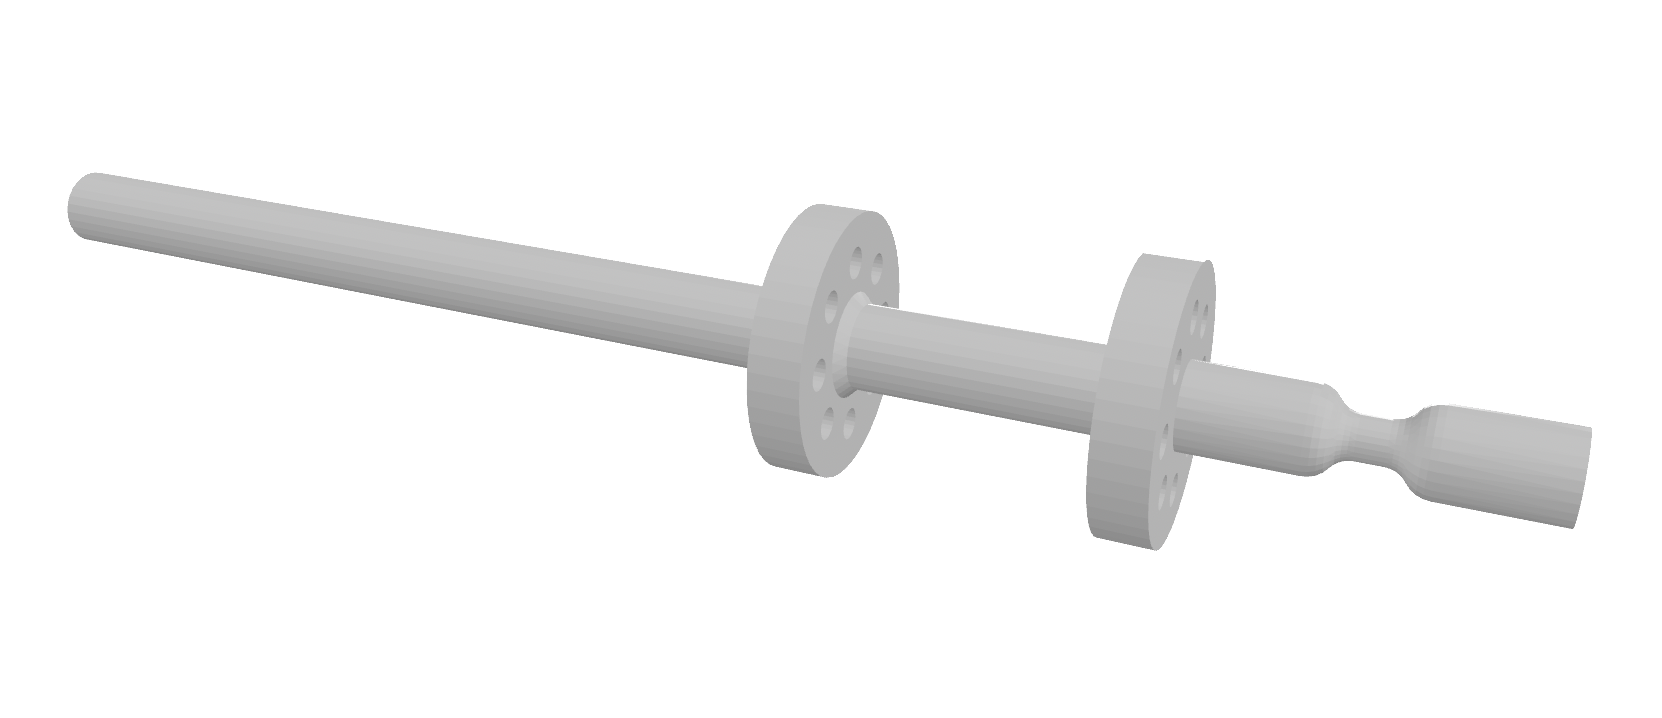
\includegraphics[width=5cm]{./figs/model_shaft.png}
%     \caption{設計に使用するモデルデータ(回転軸部)}
%     \label{kanran3}
% \end{figure}


次に，回転体の質量バランスの調整について述べる．ボタン，電池，ホルダー，そしてレーザーモジュールで構成される，レーザーによる光信号送信基盤を回転リングへ取り付ける際，当初はリング内に収まることを優先して両面テープで貼り付けていた．
しかし，この配置では回転体の質量分布に偏りが生じ，回転速度にムラが発生した．そこで，4枚の電池基板を中心軸を囲うように十字状の対称配置へ変更することで偏心を抑え，回転速度のムラを解消した．さらに，両面テープでは回転の振動により固定が緩むため，瞬間接着剤による固定へ変更し，安定性を向上させた．実装した回転リングの表面・裏面を図\ref{fig:r_kanran}に示す．

\begin{figure}[htbp]
  \centering
  \begin{minipage}{0.48\textwidth}
    \centering
    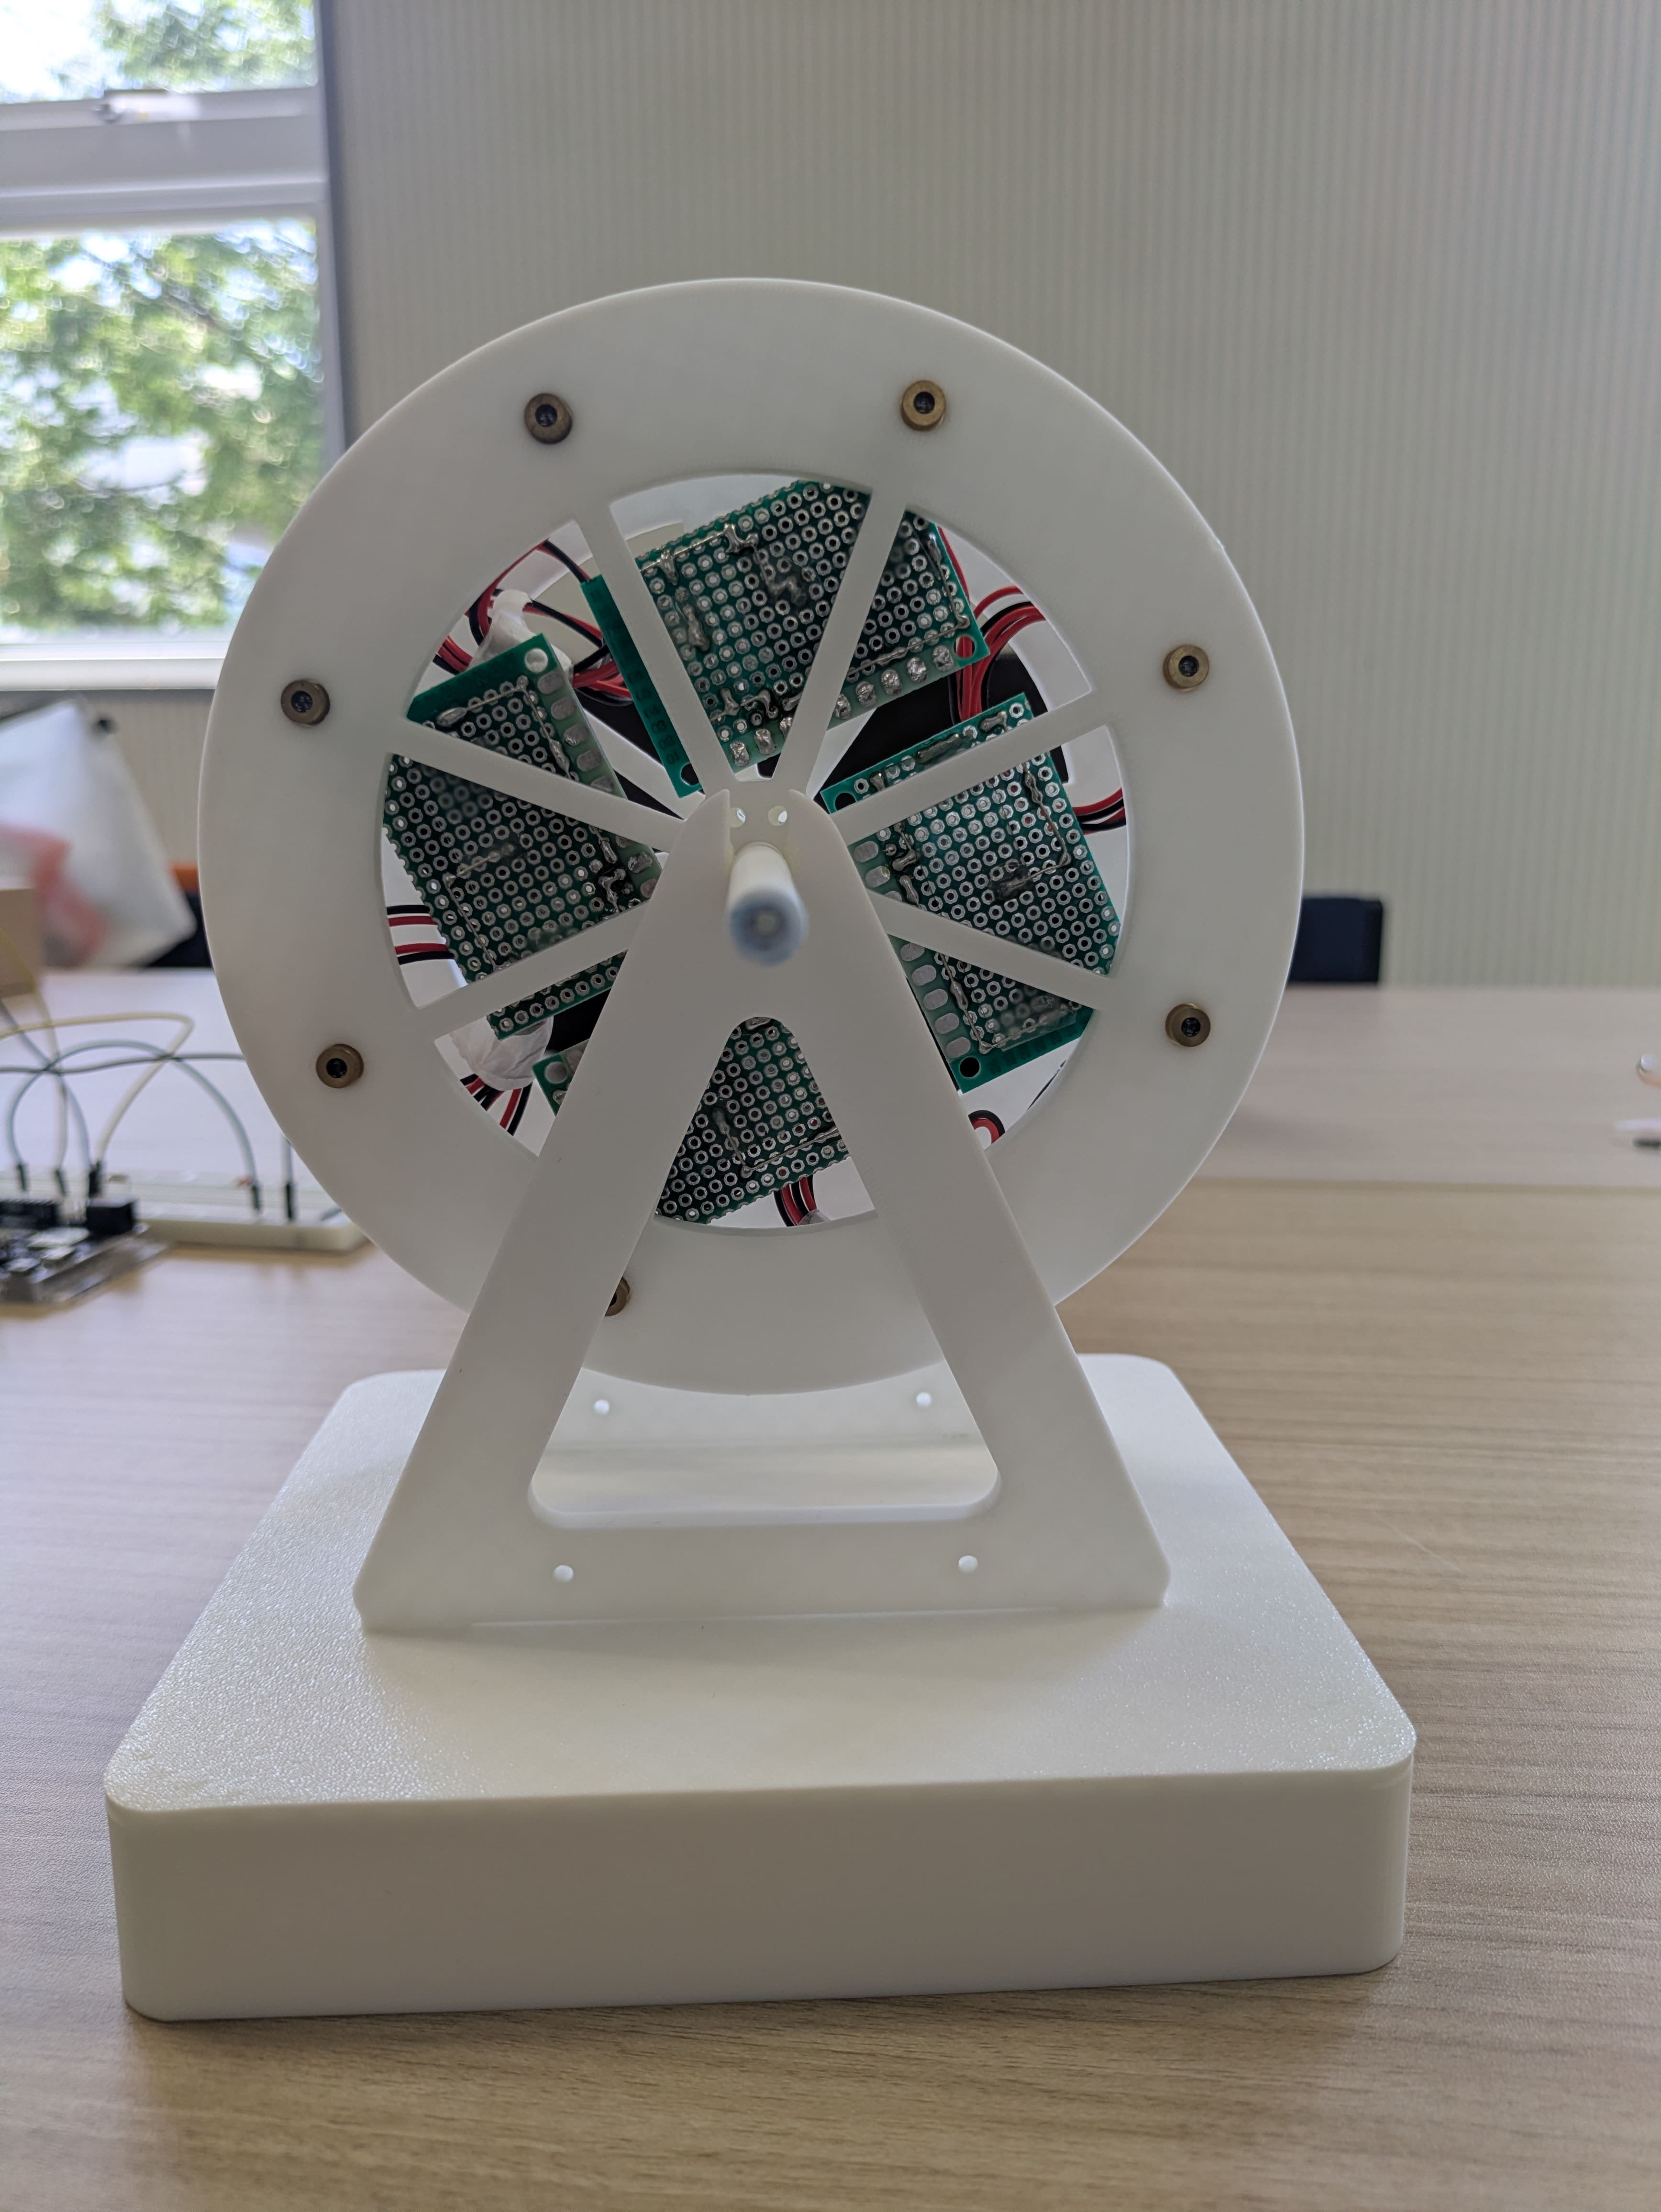
\includegraphics[width=\textwidth]{figs/R_kanranomote.jpg}
  \end{minipage}
  \hfill
  \begin{minipage}{0.48\textwidth}
    \centering
    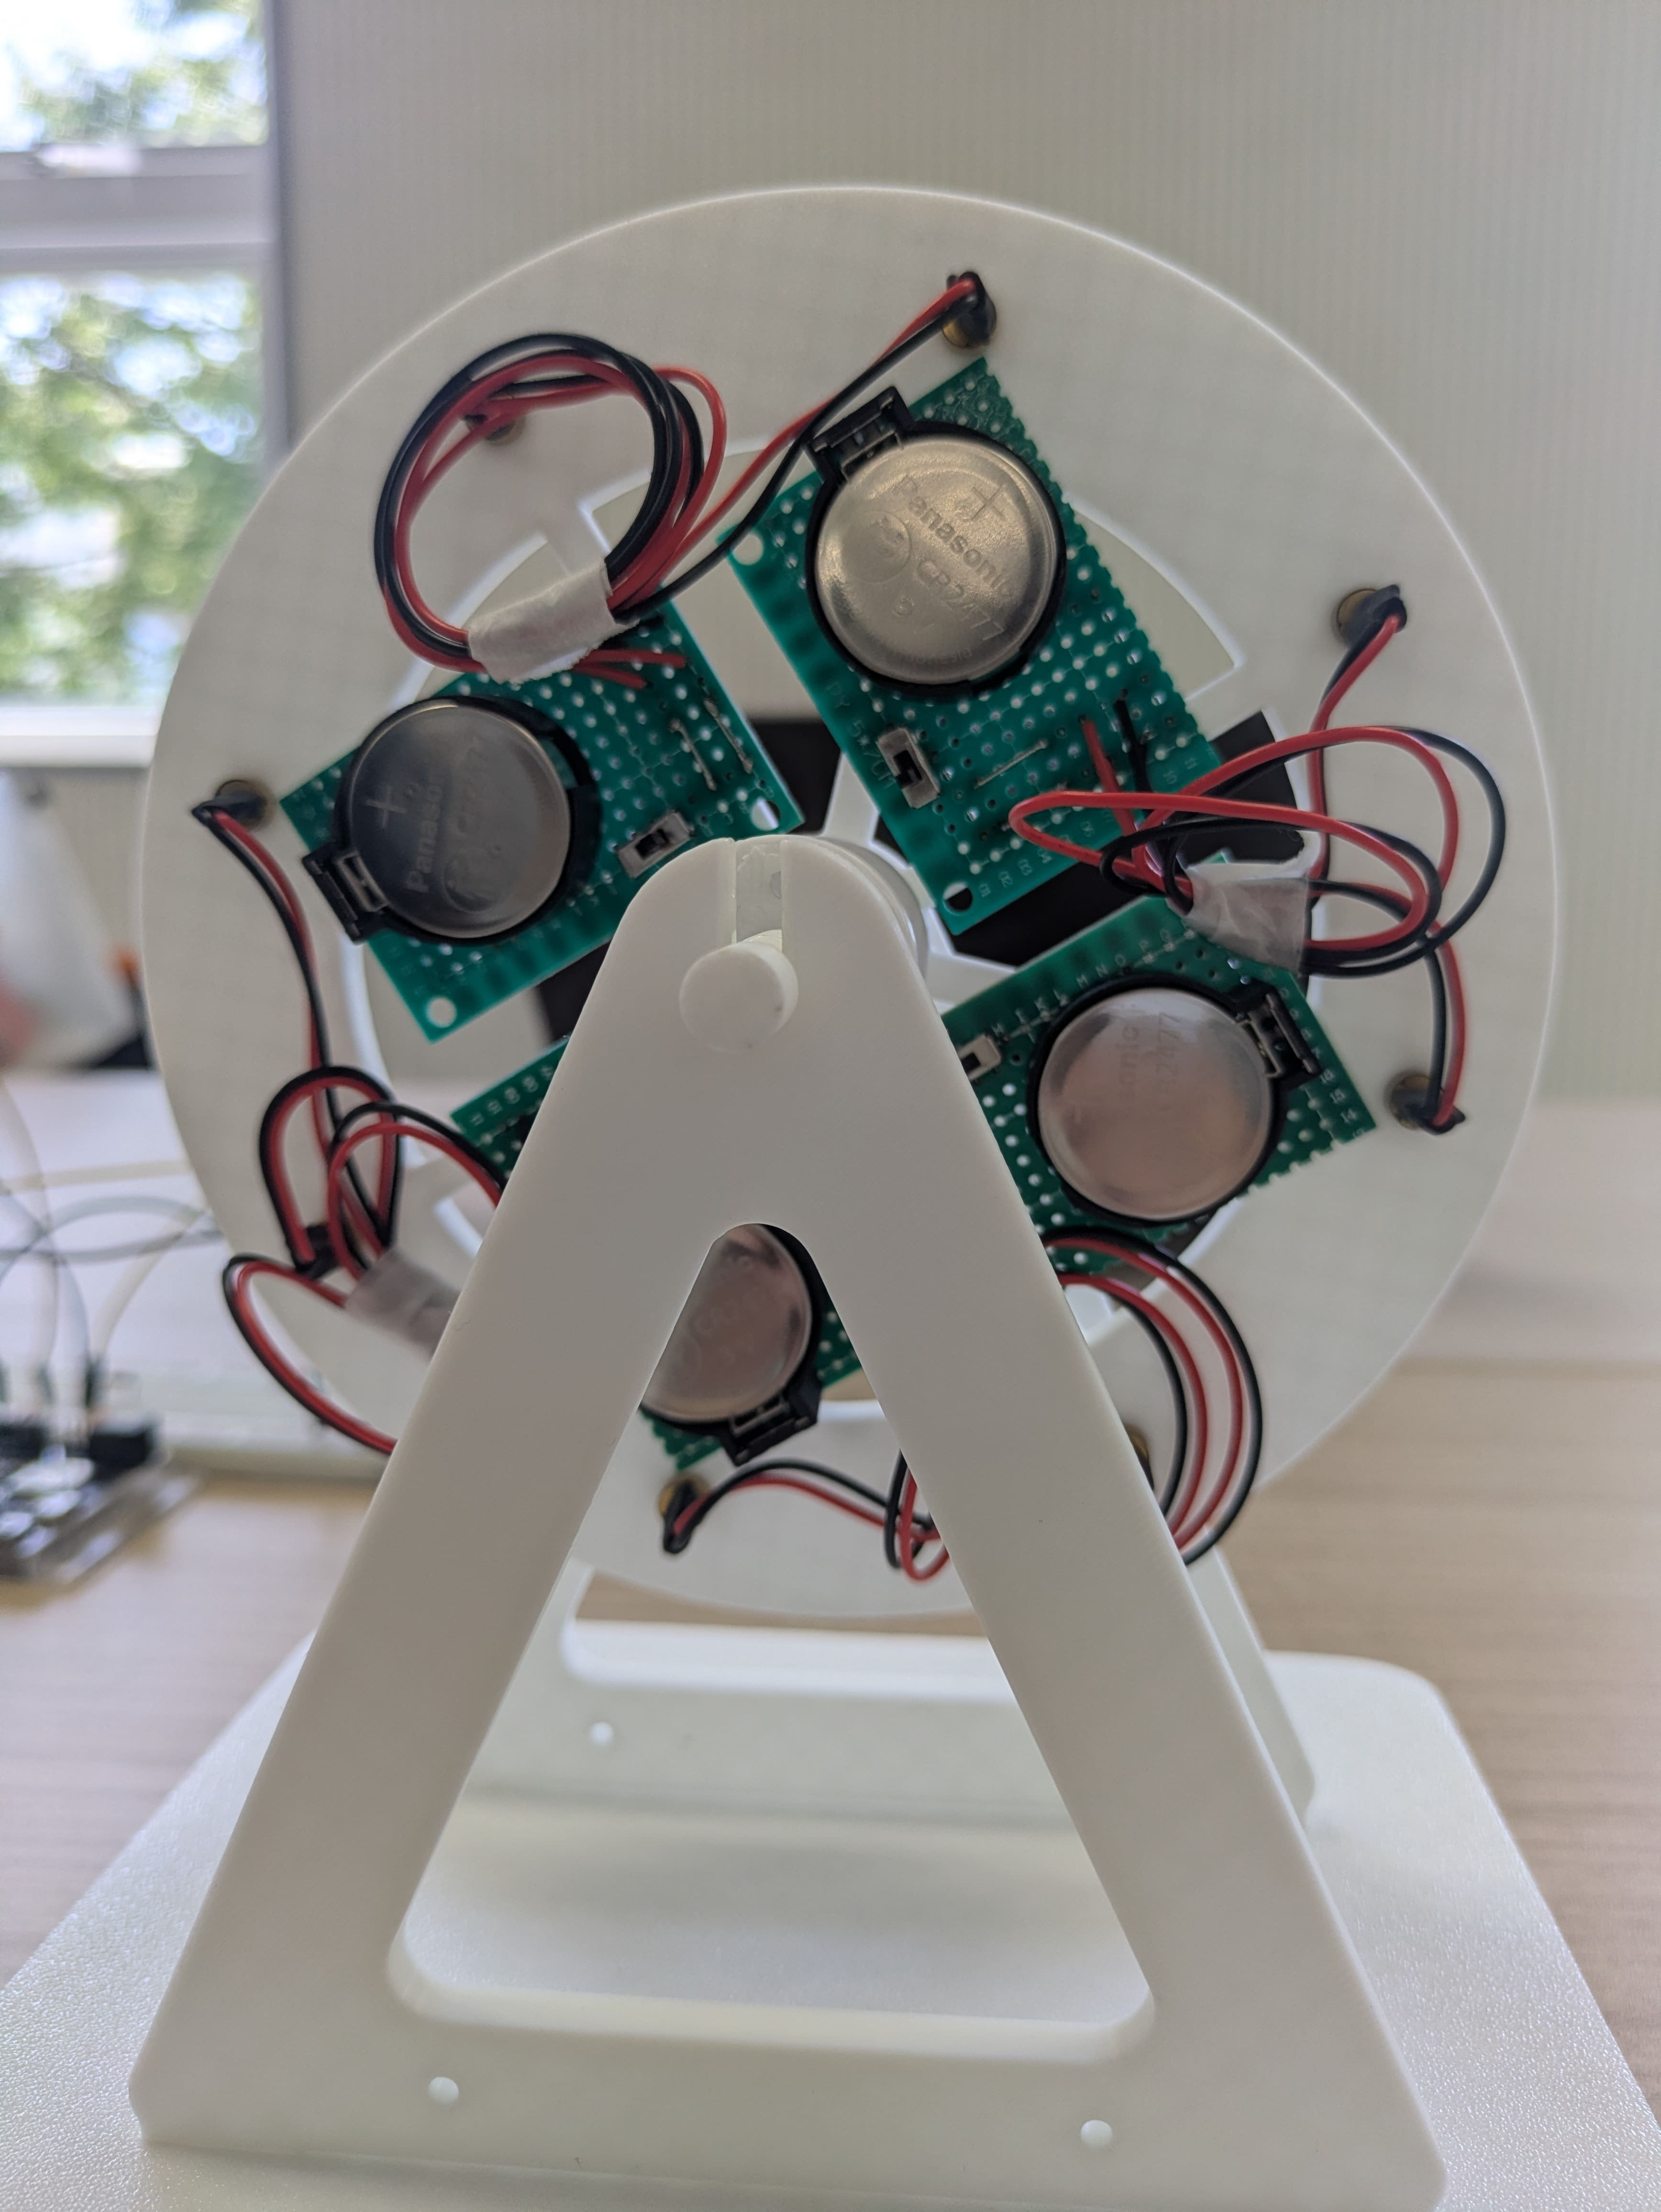
\includegraphics[width=\textwidth]{figs/R_kanranura.jpg}
  \end{minipage}
  \caption{回転リングへのレーザーによる光信号送信基板の実装（左：正面，右：背面）}
  \label{fig:r_kanran}
\end{figure}


また，動作試験の過程で，回転の反動によりモータ部が土台から浮いて動いてしまい，レーザー光の照射位置がずれて受光精度が低下する事象が確認された．この対策として，使用済みのボタン電池を土台部に載せておもりとし，モータ部の浮き上がりを抑えた．廃棄予定の電池を再利用することで，追加部品なしに質量を確保している．

さらに，動作試験を繰り返す中で，同一のPWM設定値に対するモータの回転速度が試行ごとに一定にならない事象が確認された．この要因としては，電源の起電力が試行ごとに変動していたことが考えられる．
モータの回転速度は印加電圧に依存するため，電源電圧の変動やブラシ接触抵抗の変化が回転速度の変動として現れたと考えられ，\ref{sec:kousatsu}節で述べる同期確立時間の変動要因の一つとなった可能性がある．

% 最後に，本デバイスのモータ回転制御およびLEDマトリクス表示を行う制御プログラムの全文は，付録（FerrisWheel.ino，Display.h，Display.cpp，MotorControl.h，MotorControl.cpp）に示す．

\FloatBarrier

\subsubsection{楽器デバイス受光部装置}
\label{sec:jissou_jukou}

はじめに，受光素子の選定理由について述べる．
レーザー光の検知にはCdSセルを採用した．CdSセルとは，硫化カドミウムを用いた，受光量に応じて抵抗値が変化する光導電素子である．
CdSセルは，フォトダイオード等の他の受光素子と比較して応答速度は遅いものの，抵抗値の変化を分圧回路で読み取るだけの簡素な回路で使用でき，可視光域に感度を持つためレーザーモジュール（波長\SI{650}{nm}の赤色光）の検知に適する．
本システムの受光イベントは最低でも数百 m秒であるモータの回転周期で発生するため，CdSセルの応答速度で十分であると判断した．

次に，実装における技術的貢献について述べる．
まず，レーザー光を使用する際における安全対策について述べる．レーザー光は直接目に入ると危険であるため，回転する部品と同じ大きさの阻害部品（遮光板）を製作し，レーザー光が受光部の後方へ漏れて観客の目に入ることを防止した．受光部の円盤形状は図\ref{kanran6}に示す通りである．

% \begin{figure}[htbp]
%   \centering
%   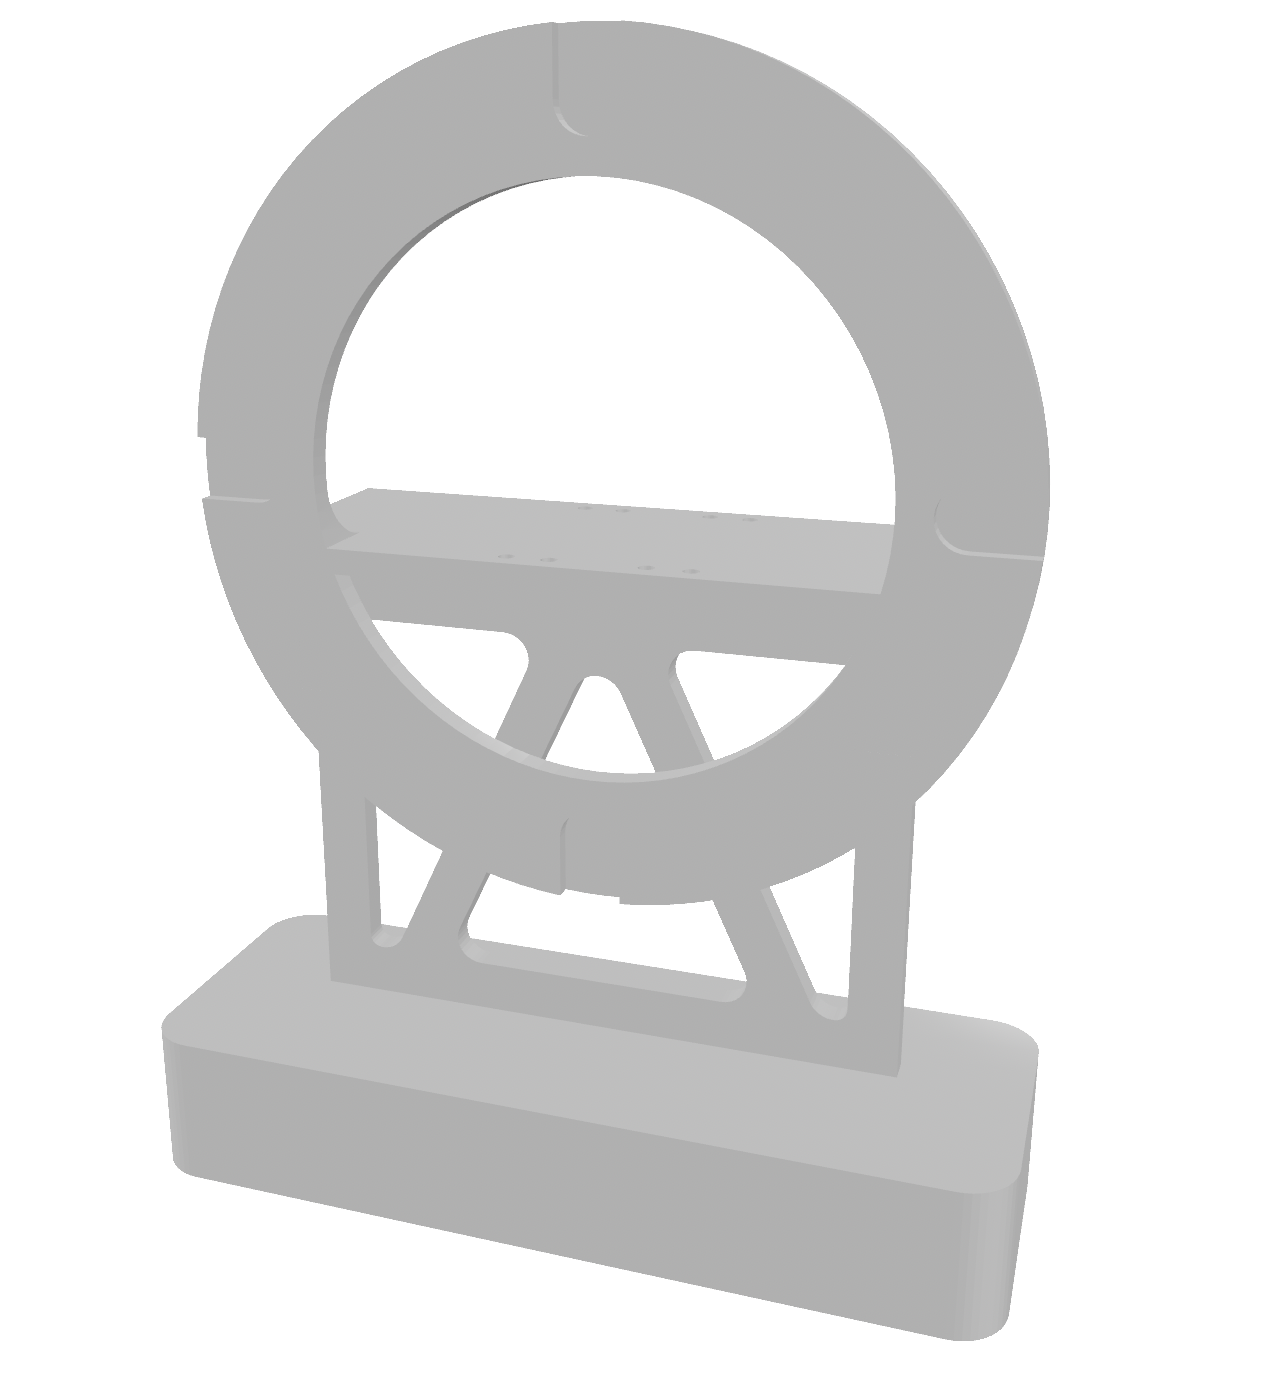
\includegraphics[width=0.45\textwidth]{figs/model_pointer.png}
%   \caption{受光部円盤の形状（3Dモデルデータ）}
%   \label{fig:jukou_daiyou}
% \end{figure}
\noindent
次に，CdSセルの設置方法について述べる．受光部の遮光板には，図\ref{kanran6}の通りCdSセルを設置するためのくぼみを90度間隔に設けている．CdSセルをこの受光部の遮光板へ固定するにあたり，当初はCdSセルを遮光板へ直接固定することを検討したが，デバイスの組み立て方やレーザー光の機微な方向の違いによって受光しやすい位置が変わり受光精度が変動するという問題があった．また，本デバイスは3Dプリンターで制作したため，ポリ乳酸(PLA)という素材特性の観点からも設置が困難である．PLAは硬度が高く寸法安定性に優れる一方で，表面が滑らかで接着剤が定着しにくいという特性を持つ．以上の観点から，CdSセルを遮光板に直接接着した場合，十分な固定強度が得られず受光精度が不安定となる問題があった．
そこで，小さく切った発泡スチロールにCdSセルの素子部分を折り曲げて沿わせ，テープで固定したうえで，この発泡スチロールごとくぼみに設置する方式とした．これにより，発泡スチロールを動かすことでCdSセルの位置を微調整でき，組み立て後にレーザー光の照射位置へ合わせ込むことが可能となった．なお，この方式で実験を続けたところ，固定していたテープが浮いてしまう事象が生じたため，テープの重ね貼りによる補強を行った．





最後に，受光精度の向上について述べる．CdSセルは受光面が小さく，回転するレーザー光の細いビームを直接受光することが困難であったため，受光精度を段階的に改善した．
まず，黒いストローでCdSセルを覆った．これは，ストローの筒内に入射したレーザー光が内部で反射してCdSセルへ届きやすくなるとともに，筒が周囲の環境光を遮ることで，受光時と非受光時の明暗差を大きくする狙いである．しかし，一般的な細さのストローでは開口部が小さく，依然として受光が困難であったため，開口径の大きいタピオカ用の黒いストローへ変更したところ，受光精度が向上した．
さらに，ストローの先端をティッシュペーパーで薄く覆うことで，レーザー光が通過する際に拡散され，ビームの位置が多少ずれても拡散光としてCdSセルへ届くようにした．加えて，ストローとCdSセルの間を瞬間接着剤で補強することで，隙間からの環境光の混入を防ぎ遮光性を高めた．実装した受光部回路を図\ref{fig:r_yomitori}に，遮光板リング全体と受光部を図\ref{fig:r_jukou}に示す．図\ref{fig:r_jukou}では，各受光部に黒いストローとティッシュペーパーによる拡散部が取り付けられ，土台部におもりとして使用済みボタン電池（黒いテープで絶縁したもの）が載せられている様子が確認できる．

\begin{figure}[htbp]
  \centering
  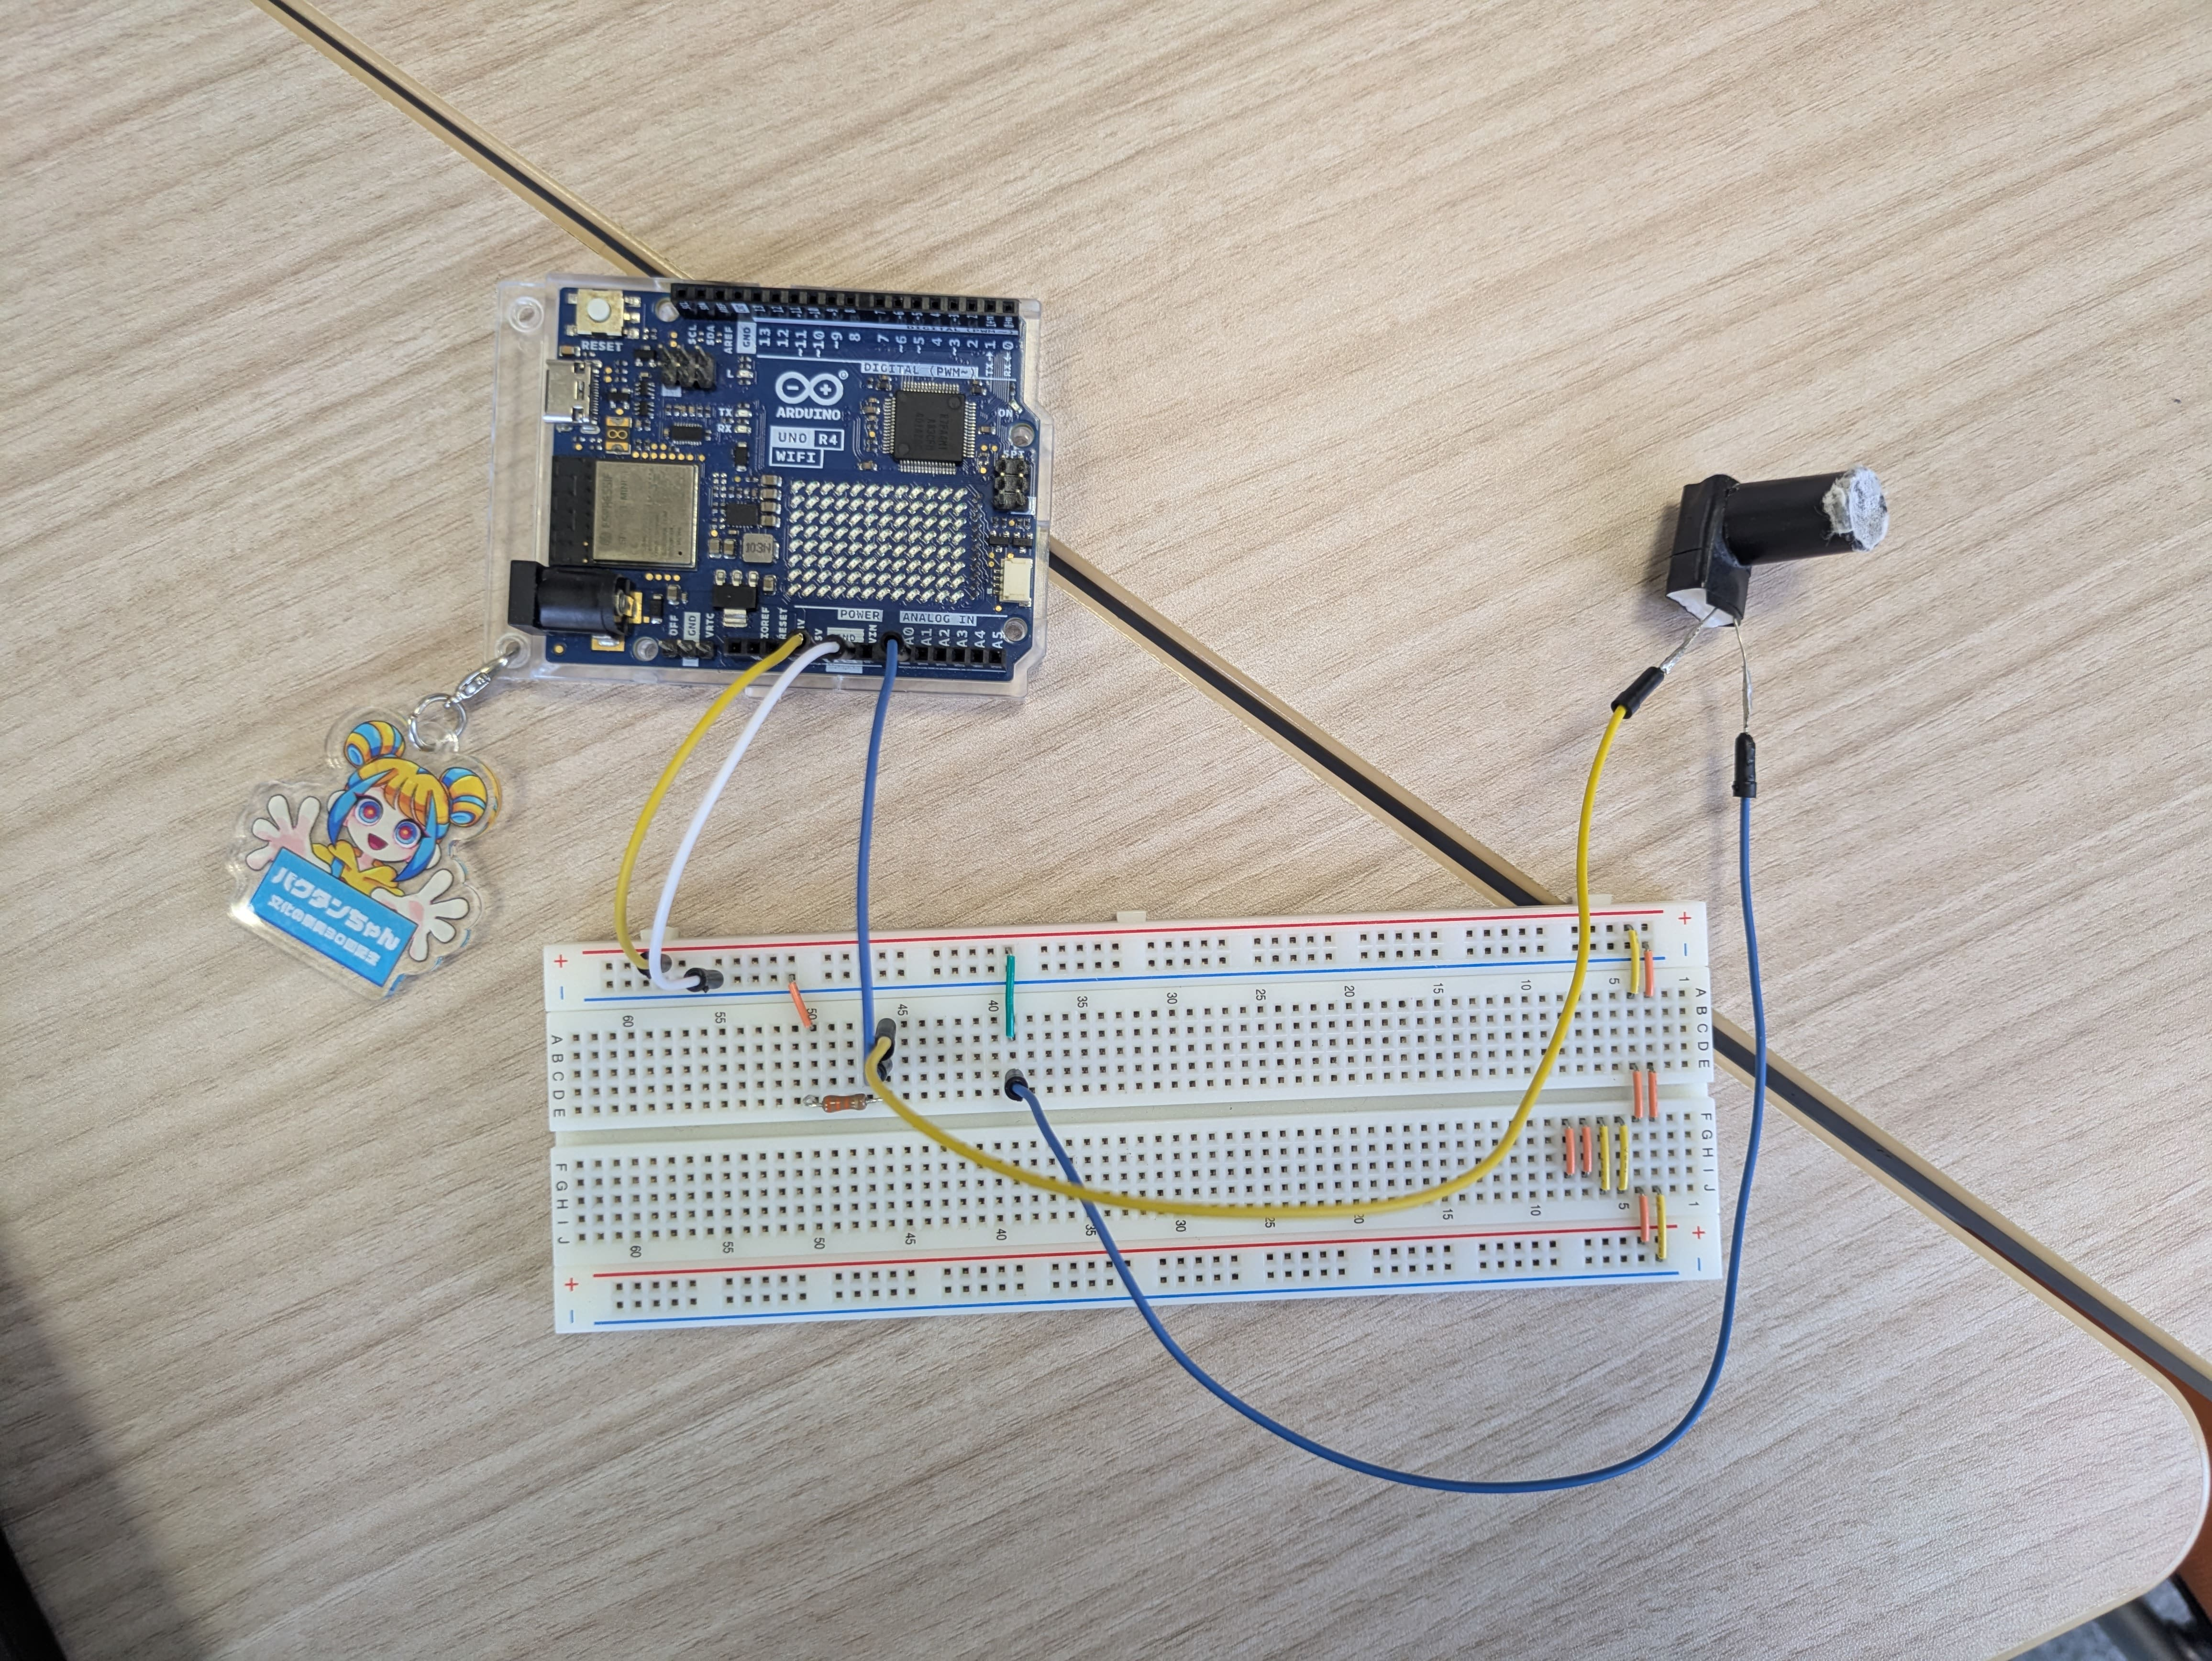
\includegraphics[width=0.6\textwidth]{figs/R_yomitori.jpg}
  \caption{受光部回路の実装}
  \label{fig:r_yomitori}
\end{figure}

\begin{figure}[htbp]
  \centering
  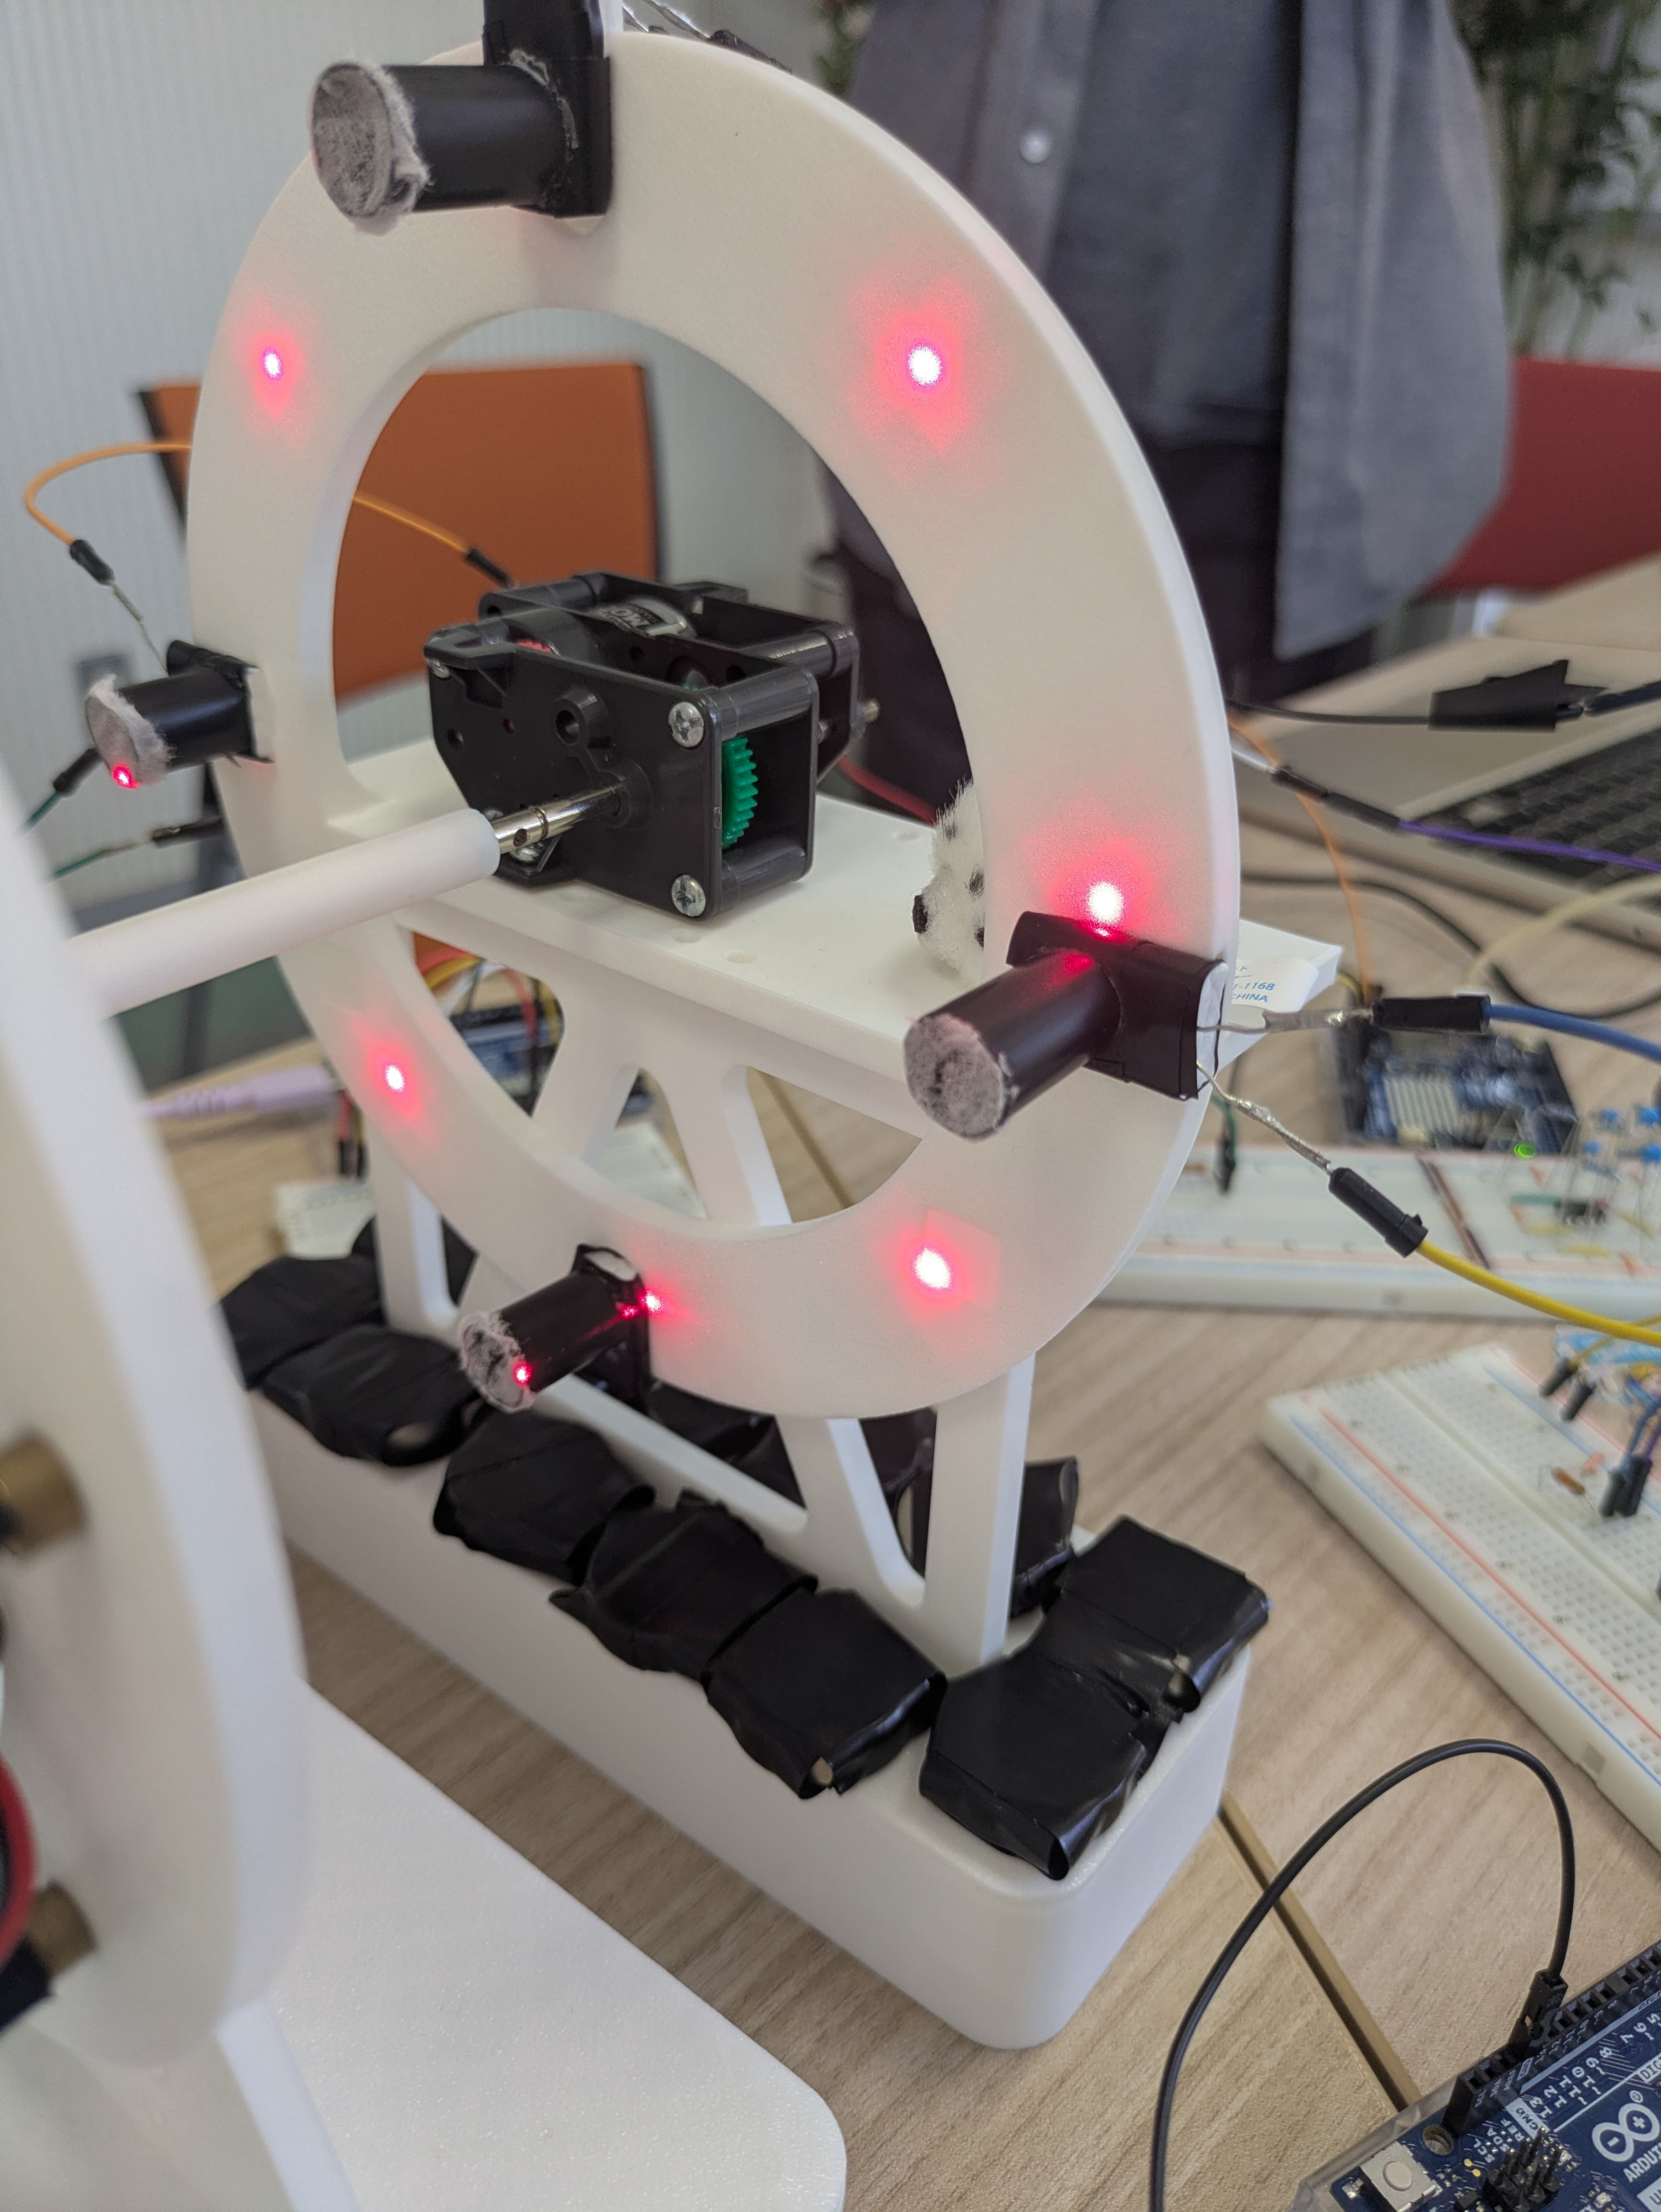
\includegraphics[width=0.7\textwidth]{figs/R_jukou.jpg}
  \caption{遮光板リングと受光部の実装}
  \label{fig:r_jukou}
\end{figure}

\FloatBarrier

\subsubsection{LEDMatrix表示プログラム}
\label{sec:jissou_display}

本節では，ソフトウェア面で担当した中継機デバイスのLEDMatrixに現在のBPMを表示するDisplayモジュール（Display.h，Display.cpp）の実装について，採用した技術の選定理由，実装の過程で直面した技術的課題，およびその解決のために行った技術的貢献を説明する．

はじめに，採用した技術とその選定理由について述べる．
第一に，数字の表示には\ref{sec:kan_naibu}項で述べた独自定義の3×5ドットフォントを採用した．これは，8行12列という限られた表示領域に最大3桁のBPM値を収めたうえで，桁間に1列の間隔を確保して可読性を保つためであり，汎用フォントライブラリを用いる方式では文字幅が大きく3桁を表示できないためである．
第二に，フレームバッファの描画方式には，設計当初に予定していた8行12列の2次元配列を直接渡す方式ではなく，96ビット分の表示内容を3個の32ビット整数へビットパックして転送する方式を採用した．これは，後者の方が描画APIへ渡すデータ量が小さくメモリ効率が高いためである．
第三に，受信データの読み込みには，設計当初に予定していた文字列としての読み込みではなく，2バイトのバイナリ形式のまま読み取り，1バイト目をヘッダ文字，2バイト目を段階番号として処理する方式を採用した．これは，\ref{sec:siki_naibu}項で述べた通信プロトコル自体が固定長2バイトのバイナリ形式で定義されており，プロトコル仕様に忠実な実装とするためである．

次に，実装の過程で直面した技術的課題とその解決について述べる．
最大の課題は，コンパイルおよび書き込みは正常に完了するにもかかわらず，LEDMatrixに何も表示されないという不具合であった．この問題の切り分けのため，起動時の点灯テストや診断用の描画処理を一時的に追加し，どの段階で表示が失われるかを段階的に確認した．その結果，原因は使用したLEDMatrix制御ライブラリの内部構造にあることが判明した．本ライブラリの表示バッファはヘッダファイル内でstatic変数として定義されているため，ヘッダを取り込んだソースファイルごとに別々の実体が生成される．このため，メインスケッチ側で初期化を行い，Displayモジュール側で描画を行う構成では，初期化と描画が互いに異なる実体に対して行われ，表示が反映されなかった．この解決として，初期化と描画を含むマトリクスへの全操作をDisplay.cpp内へ集約し，初期化用の関数（displaySetup）を新設してメインスケッチからはこれを呼び出す構成へ変更した．さらに，初期化直後の最初の描画が反映されない場合がある事象に対しては，初期化時に消灯フレームを一度描画してから\SI{200}{ms}待機するウォームアップ処理を設けることで，以降の描画を確実に反映させた．この一連の対応により，ライブラリ内部の実装に依存する不具合を，モジュール構成の見直しによって解決した．

また，設計段階の関数構成に対して，実装段階で次の機能追加を行った．演奏終了の指令（ヘッダ'E'）を受信した際にLEDMatrixを全消灯する処理は，通信プロトコル上はヘッダが定義されていたものの，設計段階の表示側関数一覧には対応する処理の記載がなかったため，消灯用の関数（clearDisplay）を追加して対応した．あわせて，桁単位の描画を行う内部関数（drawDigit）を分離することで，表示処理の見通しを改善した．

開発の経過は次の通りである．まず表示機能の骨格を作成し，設計書に沿ってBPM表示機能を実装した．この際，通信部を一時的に無効化し，与えたBPM値の描画のみを単体で検証できる状態とした．その後，前述の無表示問題の切り分けと修正を行い，表示の安定化を確認した．続いて，演奏終了時の消灯処理を追加するとともに通信部を有効化し，最後に，指揮デバイスの送信先アドレスと一致させるための静的IPアドレス設定を追加して，結合テストへ移行した．なお，開発段階では表示モジュール単体での検証のために受信処理を仮実装していたが，結合にあたっては，UDP受信を中継機デバイス本体のプログラム側で行い，Displayモジュールは描画専用とする構成に整理した．

\FloatBarrier

\subsection{開発支援ツール（生成AIを含む）の活用と検証}
\label{sec:jissou_ai}

本節では，開発過程で利用した支援ツールおよび情報源と，その利用目的・検証方法について述べる．
まず，技術情報源として，Arduino公式リファレンス，および使用した各部品のデータシートを参照した．部品の定格・接続仕様はデータシートの記載に基づいて決定し，回路実装前に確認した．
次に，生成AI（Anthropic社のClaude）を，次の3つの目的で利用した．第一に，\ref{sec:jissou_display}節で述べたLEDMatrix表示プログラムの実装補助である．第二に，評価データの統計処理およびグラフ生成用Pythonスクリプトの作成である．第三に，本稿のLaTeX原稿の草稿作成・推敲およびレイアウト調整の補助である．
LEDMatrix表示プログラムの実装では，生成AIを次の場面で利用した．実装の初期段階では，LEDMatrix制御ライブラリの利用方法や関数の仕様について質問し，実装の方針検討に用いた．ただし，回答に含まれるライブラリ名や関数名が実際の開発環境に存在しないものである場合があったため，回答をそのまま採用せず，Arduino公式リファレンスと照合して実在する名称・仕様へ修正したうえで，妥当と判断した部分のみを採用した．次に，前述のLEDMatrixに何も表示されない不具合の調査では，症状と構成を提示して原因の候補と切り分け手順の提案を受け，提案された診断手順を実機で順に実行することで，表示バッファの実体がソースファイルごとに分かれるという原因の特定に至った．このとき提案された「マトリクスへの操作を一つのソースファイルへ集約する」という修正方針は，原因の説明として整合することをコード上で確認したうえで採用した．
また，演奏終了指令の受信時に全消灯を行う処理の実装方針についても提案を受け，コンパイルと実機での表示確認により動作を検証したうえで採用した．
生成AIの出力は，次の方法で検証したうえで採否を判断した．
プログラムに関する出力については，コンパイルの成否，実機での動作，およびシリアルモニタでの出力値の確認により妥当性を検証し，さらにライブラリや関数の仕様に関する記述はArduino公式リファレンスと照合して，意図と異なる動作をする生成結果や事実と異なる記述は修正または破棄した．統計処理については，算出された統計量を教員から配布された集計シートの値と照合し，一致することを確認した．また，グラフおよび表の数値は生データからの再計算によって確認した．LaTeX原稿については，コンパイル結果の出力および図表の配置を確認するとともに，記載内容が実際の実装・測定結果と一致しているかを照合し，事実と異なる記述や根拠のない表現は修正または削除した．いずれの利用においても，生成結果をそのまま採用するのではなく，内容を理解したうえで最終的な採否と修正を判断した．

\FloatBarrier
